% Options for packages loaded elsewhere
\PassOptionsToPackage{unicode}{hyperref}
\PassOptionsToPackage{hyphens}{url}
%
\documentclass[
]{book}
\usepackage{amsmath,amssymb}
\usepackage{iftex}
\ifPDFTeX
  \usepackage[T1]{fontenc}
  \usepackage[utf8]{inputenc}
  \usepackage{textcomp} % provide euro and other symbols
\else % if luatex or xetex
  \usepackage{unicode-math} % this also loads fontspec
  \defaultfontfeatures{Scale=MatchLowercase}
  \defaultfontfeatures[\rmfamily]{Ligatures=TeX,Scale=1}
\fi
\usepackage{lmodern}
\ifPDFTeX\else
  % xetex/luatex font selection
\fi
% Use upquote if available, for straight quotes in verbatim environments
\IfFileExists{upquote.sty}{\usepackage{upquote}}{}
\IfFileExists{microtype.sty}{% use microtype if available
  \usepackage[]{microtype}
  \UseMicrotypeSet[protrusion]{basicmath} % disable protrusion for tt fonts
}{}
\makeatletter
\@ifundefined{KOMAClassName}{% if non-KOMA class
  \IfFileExists{parskip.sty}{%
    \usepackage{parskip}
  }{% else
    \setlength{\parindent}{0pt}
    \setlength{\parskip}{6pt plus 2pt minus 1pt}}
}{% if KOMA class
  \KOMAoptions{parskip=half}}
\makeatother
\usepackage{xcolor}
\usepackage{color}
\usepackage{fancyvrb}
\newcommand{\VerbBar}{|}
\newcommand{\VERB}{\Verb[commandchars=\\\{\}]}
\DefineVerbatimEnvironment{Highlighting}{Verbatim}{commandchars=\\\{\}}
% Add ',fontsize=\small' for more characters per line
\usepackage{framed}
\definecolor{shadecolor}{RGB}{248,248,248}
\newenvironment{Shaded}{\begin{snugshade}}{\end{snugshade}}
\newcommand{\AlertTok}[1]{\textcolor[rgb]{0.94,0.16,0.16}{#1}}
\newcommand{\AnnotationTok}[1]{\textcolor[rgb]{0.56,0.35,0.01}{\textbf{\textit{#1}}}}
\newcommand{\AttributeTok}[1]{\textcolor[rgb]{0.13,0.29,0.53}{#1}}
\newcommand{\BaseNTok}[1]{\textcolor[rgb]{0.00,0.00,0.81}{#1}}
\newcommand{\BuiltInTok}[1]{#1}
\newcommand{\CharTok}[1]{\textcolor[rgb]{0.31,0.60,0.02}{#1}}
\newcommand{\CommentTok}[1]{\textcolor[rgb]{0.56,0.35,0.01}{\textit{#1}}}
\newcommand{\CommentVarTok}[1]{\textcolor[rgb]{0.56,0.35,0.01}{\textbf{\textit{#1}}}}
\newcommand{\ConstantTok}[1]{\textcolor[rgb]{0.56,0.35,0.01}{#1}}
\newcommand{\ControlFlowTok}[1]{\textcolor[rgb]{0.13,0.29,0.53}{\textbf{#1}}}
\newcommand{\DataTypeTok}[1]{\textcolor[rgb]{0.13,0.29,0.53}{#1}}
\newcommand{\DecValTok}[1]{\textcolor[rgb]{0.00,0.00,0.81}{#1}}
\newcommand{\DocumentationTok}[1]{\textcolor[rgb]{0.56,0.35,0.01}{\textbf{\textit{#1}}}}
\newcommand{\ErrorTok}[1]{\textcolor[rgb]{0.64,0.00,0.00}{\textbf{#1}}}
\newcommand{\ExtensionTok}[1]{#1}
\newcommand{\FloatTok}[1]{\textcolor[rgb]{0.00,0.00,0.81}{#1}}
\newcommand{\FunctionTok}[1]{\textcolor[rgb]{0.13,0.29,0.53}{\textbf{#1}}}
\newcommand{\ImportTok}[1]{#1}
\newcommand{\InformationTok}[1]{\textcolor[rgb]{0.56,0.35,0.01}{\textbf{\textit{#1}}}}
\newcommand{\KeywordTok}[1]{\textcolor[rgb]{0.13,0.29,0.53}{\textbf{#1}}}
\newcommand{\NormalTok}[1]{#1}
\newcommand{\OperatorTok}[1]{\textcolor[rgb]{0.81,0.36,0.00}{\textbf{#1}}}
\newcommand{\OtherTok}[1]{\textcolor[rgb]{0.56,0.35,0.01}{#1}}
\newcommand{\PreprocessorTok}[1]{\textcolor[rgb]{0.56,0.35,0.01}{\textit{#1}}}
\newcommand{\RegionMarkerTok}[1]{#1}
\newcommand{\SpecialCharTok}[1]{\textcolor[rgb]{0.81,0.36,0.00}{\textbf{#1}}}
\newcommand{\SpecialStringTok}[1]{\textcolor[rgb]{0.31,0.60,0.02}{#1}}
\newcommand{\StringTok}[1]{\textcolor[rgb]{0.31,0.60,0.02}{#1}}
\newcommand{\VariableTok}[1]{\textcolor[rgb]{0.00,0.00,0.00}{#1}}
\newcommand{\VerbatimStringTok}[1]{\textcolor[rgb]{0.31,0.60,0.02}{#1}}
\newcommand{\WarningTok}[1]{\textcolor[rgb]{0.56,0.35,0.01}{\textbf{\textit{#1}}}}
\usepackage{longtable,booktabs,array}
\usepackage{calc} % for calculating minipage widths
% Correct order of tables after \paragraph or \subparagraph
\usepackage{etoolbox}
\makeatletter
\patchcmd\longtable{\par}{\if@noskipsec\mbox{}\fi\par}{}{}
\makeatother
% Allow footnotes in longtable head/foot
\IfFileExists{footnotehyper.sty}{\usepackage{footnotehyper}}{\usepackage{footnote}}
\makesavenoteenv{longtable}
\usepackage{graphicx}
\makeatletter
\def\maxwidth{\ifdim\Gin@nat@width>\linewidth\linewidth\else\Gin@nat@width\fi}
\def\maxheight{\ifdim\Gin@nat@height>\textheight\textheight\else\Gin@nat@height\fi}
\makeatother
% Scale images if necessary, so that they will not overflow the page
% margins by default, and it is still possible to overwrite the defaults
% using explicit options in \includegraphics[width, height, ...]{}
\setkeys{Gin}{width=\maxwidth,height=\maxheight,keepaspectratio}
% Set default figure placement to htbp
\makeatletter
\def\fps@figure{htbp}
\makeatother
\setlength{\emergencystretch}{3em} % prevent overfull lines
\providecommand{\tightlist}{%
  \setlength{\itemsep}{0pt}\setlength{\parskip}{0pt}}
\setcounter{secnumdepth}{5}
%\usepackage{bookdown} # THIS IS NOT NEEDED according to the creator!
\usepackage{pdfpages}  % Ensure this is added to load the pdfpages package
\usepackage{graphicx}
\usepackage[margin=1in]{geometry}
\usepackage{hyperref}
\usepackage{tikz}
\newcommand{\pandocbounded}[1]{#1}
\usetikzlibrary{arrows,shapes,backgrounds,calc,positioning,fit}
\ifLuaTeX
  \usepackage{selnolig}  % disable illegal ligatures
\fi
\usepackage[]{natbib}
\bibliographystyle{plainnat}
\IfFileExists{bookmark.sty}{\usepackage{bookmark}}{\usepackage{hyperref}}
\IfFileExists{xurl.sty}{\usepackage{xurl}}{} % add URL line breaks if available
\urlstyle{same}
\hypersetup{
  pdftitle={Quantitative Methods 1, ZHAW},
  pdfauthor={Jürgen Degenfellner},
  hidelinks,
  pdfcreator={LaTeX via pandoc}}

\title{Quantitative Methods 1, ZHAW}
\author{Jürgen Degenfellner}
\date{2024-11-01}

\begin{document}
\maketitle

{
\setcounter{tocdepth}{1}
\tableofcontents
}
\chapter{Introduction}\label{introduction}

This script is a collection of notes and exercises for the course ``Quantitative Methods 1'' (Codename for: Statistical foundations) at \href{https://www.zhaw.ch/en/university/}{ZHAW} in Winterthur, Switzerland.
It is permanently evolving and the \href{https://github.com/jdegenfellner/Script_QM1_ZHAW}{github repository} is public.

The \textbf{vision} is to write this script in \textbf{collaboration with students}. If you find any errors, have suggestions, or want to contribute, feel free to contact me.
Which (online) content (video, book, blog\ldots) helped you understand the topic at hand better? We should link those resources in the script!

The \textbf{goal} of this script is to provide a starting point for further reading and learning. It should function as an initial start to get you going. We are all learners.

Feel free to use any content for your own purposes.

At the end of each chapter, you will find a list of exercises. Last year's exam will be uploaded in time in the respective Moodle folder to help you prepare.

The most important lessons you'll learn are not part of the final exam: Intellectual honesty and humility.

A lot of content relevant for this course can be found in the \href{https://github.com/jdegenfellner/ZHAW_Teaching}{ZHAW\_teaching} folder,
which contains many R scripts (among other stuff).

We will focus a lot on descriptive statistics and basic concepts as it is a very important part of understanding data.
Statistical modeling will be covered later.

One thing to consider for health sciences with respect to quantitative methods is the following: We do not \emph{have} to use quantitative methods for each and every
question arising in applied research (physiotherapy, midwifery, nursing, occupational therapy). Small sample sizes (e.g., n=10) often do not warrant the use of inferential
statistics or estimation or at least make it considerably harder to answer the question at hand.
\emph{If} one decides to answer questions in a statistical way, we are bound to the rules of the game.

GPT4o and Github Copilot where used for writing this script.

\section{Books I can (highly) recommend:}\label{books-i-can-highly-recommend}

\begin{itemize}
\tightlist
\item
  FILL in HERE: book recommendation for Probability and descriptive statistics\ldots.
\item
  \href{https://xcelab.net/rm/}{Statistical Rethinking}, YouTube-Playlist: \href{https://youtu.be/FdnMWdICdRs?si=q2py5QVY_L299hEa}{Statistical Rethinking 2023}
\item
  (Free) \href{https://vdoc.pub/documents/understanding-regression-analysis-a-conditional-distribution-approach-84oqjr8sqva0}{Understanding Regression Analysis: A Conditional Distribution Approach}
\item
  (Free) \href{https://nyu-cdsc.github.io/learningr/assets/kruschke_bayesian_in_R.pdf}{Doing Bayesian Data Analysis}
\item
  \href{https://us.sagepub.com/en-us/nam/applied-regression-analysis-and-generalized-linear-models/book237254}{Applied Regression Analysis and Generalized Linear Models}
\end{itemize}

These books are well-written, approachable, and not overly technical.

For more theoretically advanced approaches, I can recommend:

\begin{itemize}
\tightlist
\item
  (Free) \href{http://www.stat.columbia.edu/~gelman/book/}{Bayesian Data Analysis}
\item
  (Free) \href{https://web.stanford.edu/~hastie/ElemStatLearn/}{Elements of Statistical Learning}
\item
  (Free) \href{https://students.aiu.edu/submissions/profiles/resources/onlineBook/y6z7i8_t4q6Z9_advanced\%20statistics.pdf}{Unterstanding Advanced Statistical Methods}
\end{itemize}

\section{\texorpdfstring{
\includegraphics[height=1.8ex]{images/Rlogo.png}}{}}\label{section}

In this course, we use \href{https://www.r-project.org/}{R} as our main tool for data analysis. R is a free software environment for statistical computing and graphics.
It compiles and runs on a wide variety of UNIX platforms, Windows, and MacOS.

You may want to give Hadley Wickham's book a try:

\begin{itemize}
\tightlist
\item
  (Free) \href{https://r4ds.had.co.nz/}{R for Data Science}
\end{itemize}

Especially, the chapter on \href{https://r4ds.hadley.nz/eda\#introduction}{exploratory data analysis} is very helpful.

This free book seems also very helpful for beginners:

\begin{itemize}
\tightlist
\item
  (Free) \href{https://bookdown.org/daniel_dauber_io/r4np_book/}{R for non-programmers R4NP}
\end{itemize}

Further resources:

\href{https://www.youtube.com/watch?v=V8eKsto3Ug&t=140s}{(Example) Introduction to R}

In this video, many basic commands are explained. There are many more R introductions.
My tip: Watch the beginning of a few different ones and see which explanations work best for you individually.

\href{https://cran.r-project.org/other-docs.html}{Overview of introductory resources}

\section{Additional Tools}\label{additional-tools}

Currently I use a combination of \href{https://github.com/features/copilot}{Github Copilot} (paid), \href{https://chatgpt.com/}{GPT4o} (paid), and \href{https://posit.co/download/rstudio-desktop/}{RStudio} for writing code and this script. You can use Github Copilot directly in RStudio to make code suggestions, which is often increasing productivity. I can highly recommend using these tools in combination. GPT4o can process images as well, which is a game changer.
As far as I know, there is no self-debugging version of GPT4o in combination with RStudio available yet (in the style of AutoGPT or similar approaches). Maybe, we'll work on that soon as a side project. For the more technically inclined among you,
you can also use VSCode with the Github Copilot extension to write your R-Code.

Large Language Models (LLM) like GPT4o enable you to write/adapt code using natural language. Among other tasks, they help you create complicated, aesthetic plots. Very often, debugging attempts get stuck. They are far from perfect yet, but an impressive feat of engineering.

\section{Workflow suggestion}\label{workflow-suggestion}

You could use RStudio to write and execute your code. In the global options of RStudio (below), you can add your github copilot account. Additionally, you can have your GPT4o(1) window open and copy-paste images of your plots or code in order to achieve your current objective.
\pandocbounded{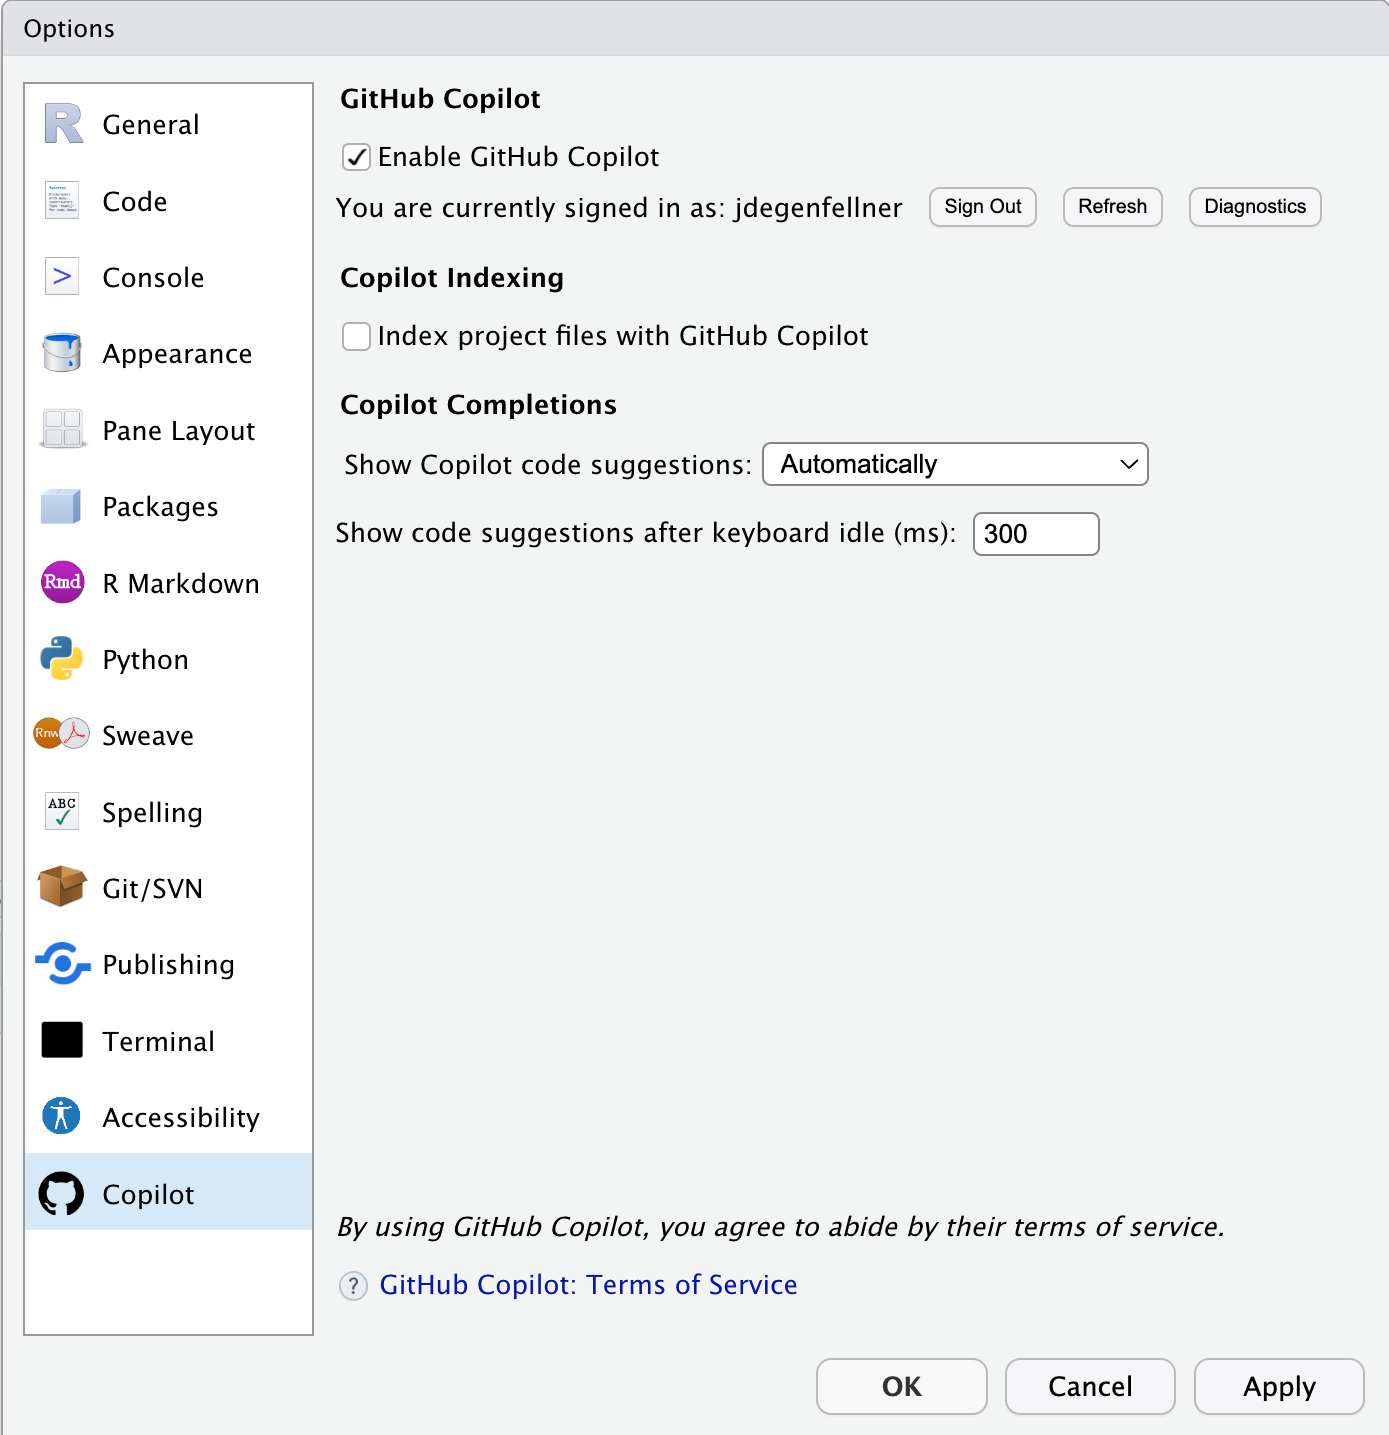
\includegraphics[keepaspectratio]{./images/RStudio_Global_Options.png}}

\chapter{Probability}\label{probs}

Probability is a measure of the likelihood that an event will occur. Probability is quantified as a number between 0 and 1 (or 0 to 100\%),
where 0 indicates impossibility and 1 indicates certainty, although we will see later that a \href{https://stats.stackexchange.com/questions/273382/how-can-the-probability-of-each-point-be-zero-in-continuous-random-variable}{probability of 0} does not necessarily mean that such an event can never occur.
The higher the probability of an event, the more likely it is that the event will occur.

\textbf{Why is probability important in our field of study (applied health sciences)?}

Quantative research methods (often a code name for statistics) use probability theory to make statements about a larger
population or a data generating process (DGP), as it should be more appropriately called.

In observational studies, we often make statements about associations between variables.

In experimental studies (e.g., a randomized controlled trial), we often try to make statements about the effect of an intervention on a
certain outcome - for instance if a therapy lowers \href{https://jamanetwork.com/journals/jama/fullarticle/2794765}{pain} by at least 1 point better compared to usual therapies.

Probability theory has its roots in gambling and betting. \href{https://en.wikipedia.org/wiki/Blaise_Pascal}{Blaise Pascal} wrote a letter to \href{https://en.wikipedia.org/wiki/Pierre_de_Fermat}{Pierre de Fermat} in 1654 when a
French essayist Antoine Gombaud, intrigued by gambling, sought to solve ``the problem of points,''
first posed by Luca Paccioli in 1494. The problem asked how to fairly divide the winnings if a game is interrupted before
its conclusion. Gombaud approached mathematician Blaise Pascal, who collaborated with Pierre de Fermat. Together, they laid
the groundwork for modern probability theory. Fermat's method involved listing all possible outcomes and calculating each player's
chance of winning, while Pascal developed a backward induction algorithm to assign probabilities. Their work revolutionized mathematics
and influenced fields like economics and actuarial science.

Philosophically speaking, we could distinguish between two flavors of probability: Probabilities for events that are repeatable respectively have already happened, and probabilities for events that haven't happened yet.

An example for a repeatable event is getting a 6 when throwing a fair die. We can do this experiment right now by fetching a die and throwing it.

An example for the latter is the probability of a patient dying within the next 5 years after a certain diagnosis.
It is hard to argue that this experiment would be repeatable under (almost) identical conditions since every patient is different whereas the dice are typically much more similar.
Here, we could at least put forward that other similar patients have a certain proportion of dying within 5 years.

There are of course events that have not happend ever before, like the creation of artificial general intelligence (\href{https://en.wikipedia.org/wiki/Artificial_general_intelligence}{AGI}).
Nevertheless, one can still try to assign probabilities \href{https://research.aimultiple.com/artificial-general-intelligence-singularity-timing/}{when} such an event would happen.

\section{Frequentist vs.~Bayesian statistics}\label{frequentist-vs.-bayesian-statistics}

There are two main schools of thought in statistics: Frequentist and Bayesian. Often one hears that there is a ``war'' \href{https://www.youtube.com/watch?v=8wVq5aGzSqY&t=22s&ab_channel=VeryNormal}{between the two}.

It is \emph{not} our place to say which one is better. Both have their strengths and weaknesses and are used in different contexts.

I would consider the rapant misuse of \href{https://www.sciencedirect.com/science/article/abs/pii/S0037196308000620?via\%3Dihub}{p-values} and the
cookbook-like application of frequentist statistics as a weakness of this approach (in its widely used form at least).
Of course, this is not the method's fault but the fault of the user.

Bayesian statistics is often considered more intuitive and flexible. It is also more computationally demanding and requires prior knowledge which is argued to be subjective.
Computation time is sometimes still an issue in comparison for instance in regression modelling when using an end user laptop.
It is also argued that for large sample size frequentist and Bayesian statistics converge to the same result.

There are very smart proponents on both sides and we will try to use and contrast both techniques throughout this script whenever convenient.

Especially one of the early eminent statisticians, \href{https://en.wikipedia.org/wiki/Ronald_Fisher}{Ronald Fisher}, was an oponent of Bayesian statistics,
or as he called it: \href{https://errorstatistics.com/wp-content/uploads/2016/02/fisher-1930-inverse-probability.pdf}{``inverse probability''}.

The only thing we are interested in is the practical application of both methods in the field of applied health sciences.
How well can we describe data and make predictions, how well can we learn from data in our field?

\subsection{Frequentist statistics}\label{frequentist-statistics}

Frequentist statistics is based on the idea that \href{https://en.wikipedia.org/wiki/Frequentist_probability}{probability} is the long-run
frequency of events. For instance, if I throw a fair die 1000 times, the frequency of getting a 3 is (approximately) \(\frac{1}{6}\). In the limit,
if I throw the die infinitely many times, the frequency of getting a 3 will converge to \(\frac{1}{6}\). In mathematical notation, we would write

\[
\mathbb{P}(\text{getting a 3}) = \lim_{n \to \infty} \frac{\text{Number of 3s in } n \text{ throws}}{n} = \frac{1}{6},
\]

where \(\mathbb{P}\) is the probability measure which we will define more formally later (see \hyperref[exercise1]{Exercise 1}).

More genereally, in frequentist statistics, we are looking for a fixed but unknown parameter from an underlying data generating process (DGP).
In the dice example, the process of repeatedly throwing the die is the data generating process.
Basically, we could estimate the parameter of interest arbitrarily well by reapeated drawing from the DGP if we had enough data.

\textbf{Example}: Throw your (fair or unfair) die often enough and you will get a good estimate of the probability of getting a 3.

\textbf{Example}: We could try to estimate the mean birth weight of all babies from smoking parents born in Switzerland in 2022.
We would draw a (random) sample of birthweights and calculate the mean. With a sample large enough, we could estimate this parameter fairly well.
With all birthweights, we would know the true mean of the population of interest (for that year alone).

\subsection{Bayesian statistics}\label{bayesian-statistics}

Bayesian statistics, on the other hand, is based on the idea that \href{https://en.wikipedia.org/wiki/Bayesian_probability}{probability} is a measure of our uncertainty about an event or a parameter.
Here, we use \emph{prior} (i.e., before/outside of our experiment) knowledge about a parameter and update this knowledge with new data using the famous Bayes' theorem:

\[
p(\theta | \text{data}) = \frac{p(\text{data} | \theta) \cdot p(\theta)}{p(\text{data})},
\]

where:

\begin{itemize}
\item
  \(p(\theta | \text{data})\) is the \textbf{posterior probability}: the updated probability of the parameter \(\theta\) given the observed data.
\item
  \(p(\text{data} | \theta)\) is the \textbf{likelihood}: the probability of observing the data given a certain value of the parameter \(\theta\).
\item
  \(p(\theta)\) is the \textbf{prior probability}: the initial belief about the parameter \(\theta\) before seeing the data.
\item
  \(p(\text{data})\) is the \textbf{marginal likelihood} or \textbf{evidence}: the probability of observing the data under all possible parameter values.
\end{itemize}

\subsubsection{Example in applied health sciences (physiotherapy)}\label{example1_physio}

Suppose you're a physiotherapist trying to estimate the probability that a new therapy improves the mobility of patients with chronic back pain (Improvement Yes/No).
You already have some prior knowledge (based on previous studies or expert opinions) that suggests the therapy works for 30\% of patients.
This is your \textbf{prior knowledge}: \(\theta = 0.30\), where \(\theta\) is the probability that the therapy is effective.
Your colleagues are not convinced that the therapy is effective and argue that the probability is 40\%.
Now, you run a small trial with 50 patients and observe that 22 of them showed a clinically relevant improvement in mobility (self-reported from the patient).
This new data (the result of the trial) \emph{updates} your belief about the effectiveness of the therapy.
Using Bayes' theorem (\hyperref[exercise2]{Exercise 2}), you combine the prior knowledge \(\theta = 0.30\) with the likelihood of the new data \(p(\text{data} | \theta)\), and you calculate
the \textbf{posterior probability}, \(p(\theta | \text{data})\), which reflects your updated belief about the effectiveness of the therapy after observing the trial data.
We could assign the probability of \(\theta = 0.3\) or \(\theta = 0.4\) equally: \(p(\theta = 0.3) = p(\theta = 0.4) = 0.5\).

Bayesian analysis allows you to update your estimates as new evidence becomes available, providing a flexible framework for decision-making in health sciences.

\section{Foundations of probability theory}\label{foundations-of-probability-theory}

We need to know some basic concepts of probability theory in order to dive in deeper. We will try to introduce them playfully and find formality as we go along.
As stated above, in the frequentist sense, we are interested in the long-run frequency of events. How often does an event occur if we repeat the random experiment many times?

\textbf{Heureka?}

Let's imagine we are in a research department with 1000 researches all trying to answer the same question:
Does the new physiotherapy work (e.g., reduce pain by 1 point better than the usual treatment)? Let's assume (unrealistically) that they are all working on this one question and they are not
talking about their experiments or their research methodology to each other (assumption of independence). The statistician in the department has calculated
(due to the variability of such treatment effects in the relevant population and theoretical considerations)
that even under the assumption of the therapy is not working \emph{at all} - \textbf{which we will assume for the time being} - , one would see an effect just \emph{by chance} in 4\% of the study results.

What would be considered a discovery under these cicumstances?

We now conduct an experiment. All 1000 ressearches are conducting a study with 50 patients to answer the same question. This is our random experiment (instead of throwing dice).
Instead of throwing a fair die, we do a round of ``research'' with 1000 researchers. You as observer
give the assignment to the researchers and come back as soon as all 1000 researeches have finished their experiments. Again, the are not taking to each other and we can
(unrealistically) assume that their results will be not influenced by each other.

\pandocbounded{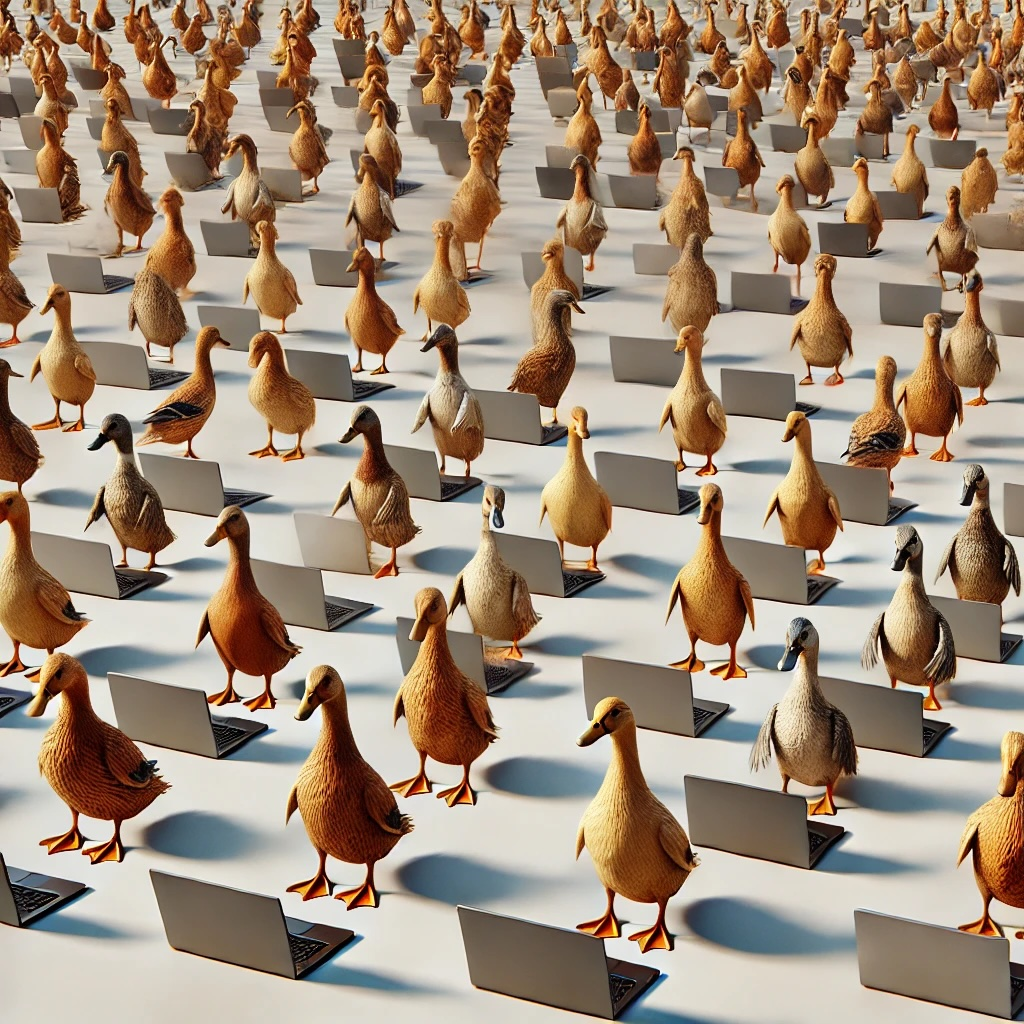
\includegraphics[keepaspectratio]{./images/thousand_researchers_ducks.jpg}}

Now we could ask different questions:

\subsection{Questions about the 1000 researcher-experiment (among many others):}\label{Questions_about_the_1000-researcher_experiment}

\begin{enumerate}
\def\labelenumi{\arabic{enumi}.}
\tightlist
\item
  If you had to bet, how many experiments showed a treatment effect if you assume that the therapy is not working at all?
\item
  If you get 137 results showing a treatment effect, would you be surprised? Would you reject the assumption, that the therapy is not working at all? Why?
\item
  How many experiments (would you expect) showed a treatment effect if you assume that the therapy is ``working'' (positive result by chance) in 12\% (instead of 4\%) of the patients?
\item
  Assuming that you have 47 results showing a treatment effect and your marketing lead is asking you to write a press release stating that 47
  out of 50 studies showed a treatment effect. What is the problem?
\item
  Assuming one very motivated researcher has tested 65 (secondary) hypotheses in her experiments and found 4 results that are difficult to explain by chance alone. What is the problem?
\item
  Suppose there are many large research departments in the world with 1000 researchers. How strongly would the number of positive results vary between these large departments?
\end{enumerate}

We will try to answer these questions \hyperref[Answers_Questions_about_the_1000-researcher_experiment]{below}.

First, it seems intuitive that Probability \emph{within} an experiment should add up \emph{if} the events are \textbf{disjoint}.
The event \(A_1=\) ``only researcher 45 gets a positive result'' and \(A_2=\) ``only researcher 897 gets a positive result'' are mutually exclusive.
If only researcher 45 finds an effect, then researcher 897 does not find an effect and vice versa. They cannot happen at the same time within that one
experiment. Hence, the two events are said to be disjoint.
If we add up the probabilities of all mutually exclusive events, we should get 1, or 100\%.
We say that the probability of all elementary events (called \(\omega\)) sums to 1. Let's look at a \href{https://en.wikipedia.org/wiki/Venn_diagram}{Venn diagram} to illustrate the concept of being mutually exclusive (disjoint).

\pandocbounded{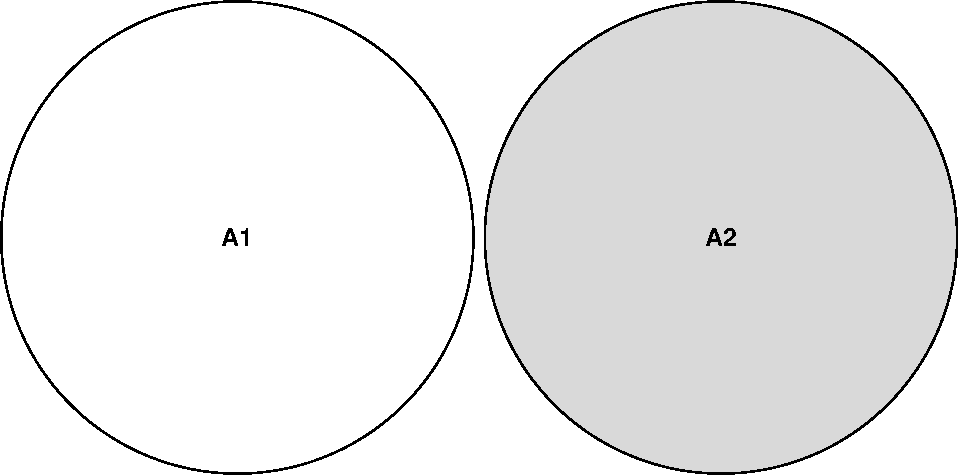
\includegraphics[keepaspectratio]{_main_files/figure-latex/unnamed-chunk-2-1.pdf}}

Again, this refers to being mutually exclusive within our 1000-researcher experiment.
Both events cannot happen at the same time in this context, so we assign \(0\) to the event that both occur simultaneously: \(\mathbb{P}(A_1 \cap A_2)=0\). The \(\cap\)-Symbol refers to all elementary events
that are in both \href{https://en.wikipedia.org/wiki/Set_(mathematics)}{sets}. In our case we have the sets

\[A_1 = \{ (\dots ,R_{45} = pos, \dots ,R_{897} = neg, \dots) \}\]

\[and\]

\[A_2 = \{ (\dots ,R_{45} = neg, \dots , R_{897} = pos, \dots) \}.\]

An example of \textbf{non-disjoint} events (within our 1000-researcher experiment) would be the event \(A_1=\) ``only researcher 45 gets a positive result'' and
the event \(A_3=\) ``only researcher 45 or only reasearcher 67 gets a positive result''.
Which researchers got a positive result in both events? The answer is: Researcher 45. Hence, the two events are said to be non-mutually exclusive. We can't just
add up the probabilities (of events \(A_1\) and \(A_3\)) here, since we would count the probability of researcher 45 twice.
The sets look like this:

\[A_1 = \{ (\dots ,R_{45} = pos, \dots) \}\]

\[and\]

\[A_3 = \{ (\dots ,R_{45} = pos, \dots), (\dots ,R_{67} = pos, \dots) \}.\]

\pandocbounded{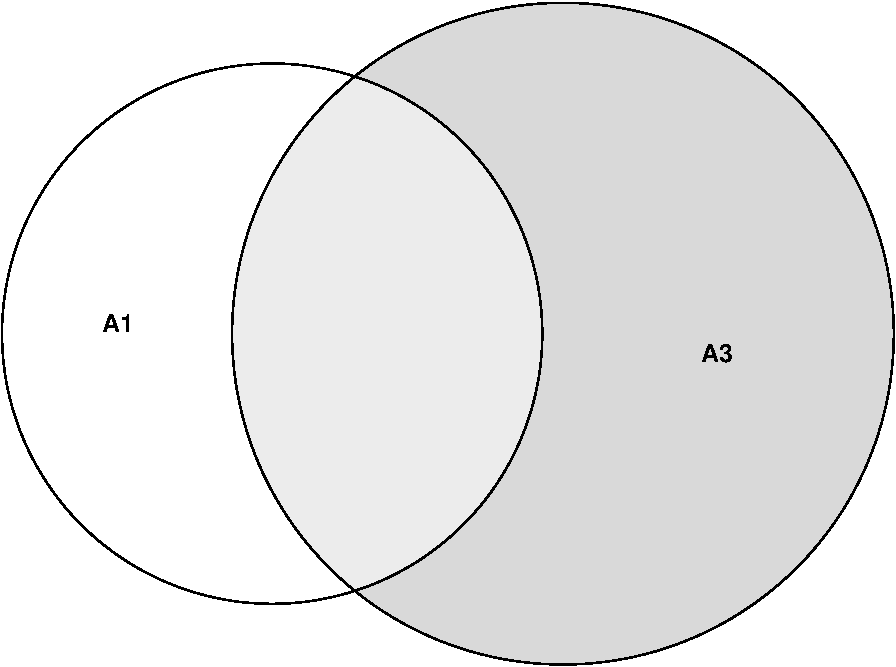
\includegraphics[keepaspectratio]{_main_files/figure-latex/unnamed-chunk-3-1.pdf}}

How many elementary events are in the set of all possible outcomes of our 1000-researcher experiment? For every researcher, there are two possible outcomes: positive or negative result.
Hence, we have \(2 \cdot 2 \cdot 2 \cdots = 2^{1000}\) elementary events in our set of all possible outcomes.
This is a very large number (\(\sim 10^{300}\)) - more than there are particles in the universe (\(\sim 10^{80}\)).

We call the set of all elementary events \(\Omega\) (the Greek letter Omega):
\[\Omega = \{ \omega_1, \omega_2, \cdots, \omega_{2^{1000}} \}.\]

Note, that \textbf{we collect elementary events to form events} like we just did for event \(A_3\).

Note, that the \textbf{\(2^{1000}\) elementary events in the 1000 researcher experiment are also disjoint}. Why? For every elementary event,
certain researchers found something and others did not. The combinations are all different from each other. Hence,
all the elementary events cannot happen at the same time within that one experiment. All of them are disjoint.

The probability of the event ``\,'' (nothing occurred) should be zero (\(\mathbb{P}(\emptyset)=0\)), were ``\,'' denotes
the event that no researcher gets a positive or negative result ( = \(\emptyset\), the so-called empty set).
This is impossible due to the design of the experiment.
We would therefore define this probability as zero and (if we can count the number of different outcomes)
this event can indeed \emph{never} happen.

Obviously, the probability of an event should at a mininum be zero and at a maximum be one:

\[0 \le \mathbb{P}(A) \le 1\].

\subsection{Axioms of probability theory}\label{axioms_of_probability_theory}

We can summarize these informally stated properties more formally (\href{https://altexploit.wordpress.com/wp-content/uploads/2017/07/a-n-kolmogorov-foundations-of-the-theory-of-probability-chelsea-pub-co-1960.pdf}{Kolmogorov's axioms}):

\begin{align}
1. &\ \mathbb{P}(\emptyset) = 0 \text{: Probability of the "impossible" event should be zero.}\\
2. &\ \mathbb{P}(\Omega) = 1 \text{: Probability, that any outcome occurs in our random experiment.}\\
3. &\ \text{If } A_1, A_2,... \text{ pairwise disjoint: } \mathbb{P}\left(\bigcup_{i=1}^{\infty} A_i\right) = \sum_{i=1}^{\infty} \mathbb{P}(A_i)
\end{align}

The \(\infty\)-symbol in \textbf{axiom 3} comes into play if we are dealing with (potentially) infinitely many events.
For instance, we could ask for the number of researchers we need to look at until we see the first
positive result (\href{https://en.wikipedia.org/wiki/Geometric_distribution}{geometric distribution}).
We could find the first positive result in the first researcher, or the second, etc. There is no upper limit.

As concrete example for law 3 in our example, we can put the following:
\begin{align}
\scriptsize \mathbb{P}(\text{"(only) researchers 34, 56 and 777 get a pos. result" or "(only) researchers 1 and 5 get a pos. results"}) =\\
\scriptsize \mathbb{P}(\text{"(only) researchers 34, 56 and 777 get a pos. result"}) + \mathbb{P}(\text{"(only) researchers 1 and 5 get a pos. results"})
\end{align}

Since the researchers are working independently from each other, we can simply multiply the probabilities of their individual positive or negative results in
our larger 1000-researcher experiment. For example, for the first probability there are exactly 3 positive results (=effect found) and 997 negative results (=no effect found).
This can be calculated as:
\(0.04 \cdot 0.04 \cdot 0.04 \cdot \underbrace{0.96 \cdots 0.96}_{\text{997 times}} = 0.04^3 \cdot 0.96^{997}\), which yields a very small number (\(1.350826 \cdot 10^{-22}\))
since we are fixating on specific researchers to find the effect.
If we relax the question to the \emph{number of researchers} that find an effect,
we get much larger numbers. We say, the number \(X\) of positive results under \(H_0\) (there is no true effect)) for a positive effect is \textbf{binomially distributed}: \(X \sim Bin(n=1000, p=0.04)\).
The YouTube-channel \href{https://www.youtube.com/@3blue1brown}{3Blue1Brown} is highly recommended in general. You should watch this
\href{https://www.youtube.com/watch?v=8idr1WZ1A7Q&ab_channel=3Blue1Brown}{video} on the binomial distribution to get a clearer picture.
This \href{https://www.youtube.com/watch?v=WWv0RUxDfbs&ab_channel=KhanAcademy}{video} from \href{https://www.youtube.com/@khanacademy}{KhanAcademy} could also be helpful.
In our example, the probability that exactly 3 researchers find an effect is \(\binom{1000}{3} \cdot 0.04^3 \cdot 0.96^{997} = 2.244627 \cdot 10^{-14}\).
Still small, but much higher than before. Of course, the commands in R can be found easily via Google or your favourite large language model (LLM):
``Give me the commands for the binomial distribution in R and a nice example too''.
Note that the sum of all elementary events (all possible outcomes) indeed adds up to 1 in our 1000-researcher-experiment: \(\sum_{i=0}^{1000} \binom{1000}{i}0.04^i 0.96^{1000-i} = 1\)

\begin{Shaded}
\begin{Highlighting}[]
\FunctionTok{sum}\NormalTok{(}\FunctionTok{dbinom}\NormalTok{(}\DecValTok{0}\SpecialCharTok{:}\DecValTok{1000}\NormalTok{, }\AttributeTok{prob =} \FloatTok{0.04}\NormalTok{, }\AttributeTok{size =} \DecValTok{1000}\NormalTok{))}
\end{Highlighting}
\end{Shaded}

\begin{verbatim}
## [1] 1
\end{verbatim}

As we will see later, \textbf{axiom 1} above does not mean, that the event can never occur.
For every continuous random variable (e.g.~with a \href{https://en.wikipedia.org/wiki/Normal_distribution}{normal}
or a \href{https://en.wikipedia.org/wiki/Continuous_uniform_distribution}{uniform distribution}), the probability of a single point is zero.
This \href{https://www.youtube.com/watch?v=ZA4JkHKZM50&list=PLIhj5_pQwhMQfGZNQZREjDdJRt0t0sn51&index=10&ab_channel=3Blue1Brown}{video} could help.

\textbf{Axiom 2} is always true. Some result \emph{has} to occur in our random experiment.
What is \(\Omega\) again? In our countable case of researchers, \(\Omega = \{ \omega_1, \omega_2, \cdots, \omega_{2^{1000}} \}\) would be the set of all possible outcomes if we let 1000 researchers conduct the experiment.
Each researcher can either find an effect or not. Hence, we have \(2^{1000}\) possible outcomes of our 1000-researcher experiment. This is a \emph{very} large number. Adding up all
these probabilities would sum to 1 according to axiom 3. Combining different elementary events \(\omega\) from the whole collection of possible outcomes \(\Omega\)
gives us ``events'' like the ones we used above (\(A_1, A_2, A_3\)).

Note that there is a \textbf{difference between the elementary experiment of the individual researcher (finding an effect or not) and the whole experiment} of
1000 researchers we are looking at (simulatenously).
Do not make the mistake to add the single probabilities of finding an effect (under \(H_0\)) of 0.04 to get the probability of finding an effect in the whole experiment:
This would result in: \(1000 \cdot 0.04 = 40 > 1\), which is hardly a probability anymore.

This leads us to the concept of independence of events.

\subsection{Independence of events}\label{independence-of-events}

Two events \(A\) and \(B\) are independent if the occurrence of one event does not affect the occurrence of the other event. In plain English,
the probability of event \(A\) happening is the same whether event \(B\) happens or not. Mathematically, we can write this as:

\[\mathbb{P}(A \cap B) = \mathbb{P}(A) \cdot \mathbb{P}(B)\] or equivalently:
\[\mathbb{P}(A | B) = \mathbb{P}(A).\]

A simple \textbf{example in our context}:
The probability of researcher 45 finding an effect (event A) is the same whether researcher 67 finds an effect (event B) or not since they are not communicating with each other.

Here, we used the very important concept of \textbf{conditional probability}.
The probability of event \(A\) \emph{given} that event \(B\) has occurred (not necessarily chronologically different!) is denoted as

\[\mathbb{P}(A | B) = \frac{\mathbb{P}(A \cap B)}{\mathbb{P}(B)}.\]

This \href{https://www.youtube.com/watch?v=ibINrxJLvlM&ab_channel=Dr.TreforBazett}{video} explains it well.

\pandocbounded{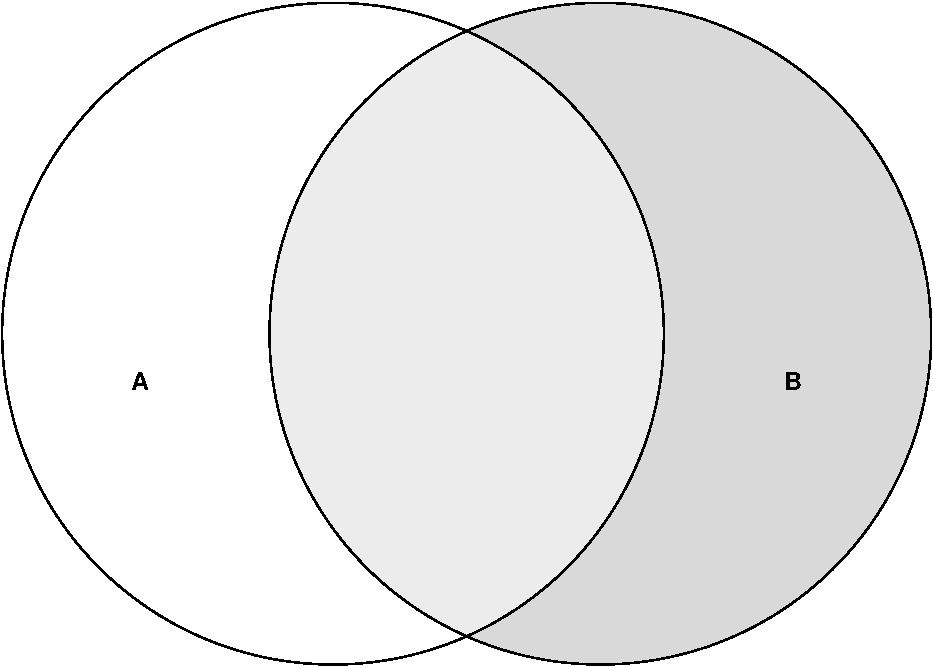
\includegraphics[keepaspectratio]{_main_files/figure-latex/unnamed-chunk-5-1.pdf}}

For the probability of event A, we a now only interested in the light-grey area with respect to the whole area of event B since event B
is our reference frame now (as opposed to the whole space \(\Omega\) before).
Note that even if the probability of event A changes when B has happend, B could still have no \emph{causal} effect on A. They could have a common cause, for instance.

\textbf{Example in our context}:
Let's assume researchers 45 and 67 would not be independent. We would for instance find that the probability of 45 is higher than 4\% if we knew that 67 found the effect.
This does not necessarily mean that researcher 67 causes researcher 45 to find an effect. It could
might as well be that their statistical training was very similar and they both made the same mistake in their analysis.

\subsection{Difference between independence and disjointness}\label{difference-between-independence-and-disjointness}

There are four possible scenarios when considering two events:

\textbf{Example 1: disjoint but not independent}

\begin{itemize}
\tightlist
\item
  Event A: Patient receives treatment A.
\item
  Event B: Patient receives treatment B (or is in the control group).
\end{itemize}

These two events, A and B, are disjoint because a patient cannot receive both treatments at the same time. If a patient receives treatment A, they cannot receive treatment B (and vice versa), meaning the events cannot occur together in this setting. Thus, \(P(A \cap B) = 0\).
However, these events are not independent, because the probability of receiving one treatment depends on not receiving the other.
In this setup, if the patient received treatment A, the probability of receiving treatment B is zero: \(\mathbb{P}(B|A) = 0\).
The probability of the patient receiving therapy B could be 50\% (if randomized): \(\mathbb{P}(B) = 0.5\). Hence, they are dependent.

\textbf{Example 2: independent but not disjoint}

\begin{itemize}
\tightlist
\item
  Event A: The patient shows a treatment effect during a study.
\item
  Event B: The patient wins the lottery during the study.
\end{itemize}

These two events are independent because the probability of a patient showing a treatment effect is not influenced by whether they win the lottery or not
(at least if we assume that lottery participants do not have different properties compared to non-lottery particiants that are conducive to showing a treatment effect).
Also, the probability of winning the lottery is not influenced by whether the patient shows a treatment effect or not. We would probably see a surge
in volunteers in our studies.
The events are unrelated: one depends on the treatment, while the other is purely a matter of luck.
However, these events are not disjoint because both can happen at the same time.
A patient could experience the treatment effect and also win the lottery during the study. Thus, \(P(A \cap B) \neq 0\) , meaning both events can occur together.

\textbf{Example 3: neither independent nor disjoint}

\begin{itemize}
\tightlist
\item
  Event A: The patient shows a treatment effect during a study.
\item
  Event B: The patient is a heavily motivated and self-sufficient.
\end{itemize}

These two events are neither independent nor disjoint. The patient's motivation could influence the treatment effect (if for instance home exercises
are part of the therapy), making the events dependent.
However, the patient's motivation is not mutually exclusive with the treatment effect: The patient can be heavily motivated and show a
treatment effect at the same time.
Hence, the events are not disjoint either. They can occur together.

\textbf{Example 4: independent and disjoint}

See \hyperref[exercise4]{Exercise 4}.

\subsection{Answers to questions about the 1000 researcher-experiment (among many others):}\label{Answers_Questions_about_the_1000-researcher_experiment}

Maybe, we can already answer some of the \hyperref[Questions_about_the_1000-researcher_experiment]{questions from above} using what we have learned so far.

\textbf{For the first question} we would probably bet on the maximum probability of the binomial distribution. The number of positive experiments out of \(1000\) has to be between \(0\) and \(1000\).
Each one of them has \(0.04\) probability of happening. With R, we quickly calculate the maximum probability:

\begin{Shaded}
\begin{Highlighting}[]
\CommentTok{\# Calculate the maximum probability using binomial distribution}
\NormalTok{n }\OtherTok{\textless{}{-}} \DecValTok{1000}  \CommentTok{\# number of researchers}
\NormalTok{p }\OtherTok{\textless{}{-}} \FloatTok{0.04}  \CommentTok{\# probability of a treatment effect for each researcher}

\CommentTok{\# Calculate the probabilities for each possible number of positive results}
\NormalTok{probs }\OtherTok{\textless{}{-}} \FunctionTok{dbinom}\NormalTok{(}\DecValTok{0}\SpecialCharTok{:}\NormalTok{n, }\AttributeTok{size =}\NormalTok{ n, }\AttributeTok{prob =}\NormalTok{ p)}

\CommentTok{\# Find the number of experiments with the highest probability}
\CommentTok{\# index of the maximum probability starting with 1}
\NormalTok{max\_prob\_number }\OtherTok{\textless{}{-}} \FunctionTok{which.max}\NormalTok{(probs)}

\CommentTok{\# Show the result}
\NormalTok{max\_prob\_number }\SpecialCharTok{{-}} \DecValTok{1} \CommentTok{\# since we started with 0}
\end{Highlighting}
\end{Shaded}

\begin{verbatim}
## [1] 40
\end{verbatim}

\begin{Shaded}
\begin{Highlighting}[]
\CommentTok{\# 40 is the most likely number of positive results}
\FunctionTok{dbinom}\NormalTok{(}\DecValTok{39}\SpecialCharTok{:}\DecValTok{41}\NormalTok{, }\AttributeTok{size =} \DecValTok{1000}\NormalTok{, }\AttributeTok{prob =} \FloatTok{0.04}\NormalTok{)}
\end{Highlighting}
\end{Shaded}

\begin{verbatim}
## [1] 0.06417798 0.06424483 0.06267788
\end{verbatim}

Now, let's visualize the binomial distribution for this case using base R syntax:

\begin{Shaded}
\begin{Highlighting}[]
\CommentTok{\# Plot the binomial distribution}
\FunctionTok{plot}\NormalTok{(}\DecValTok{0}\SpecialCharTok{:}\NormalTok{n, probs, }\AttributeTok{type =} \StringTok{"h"}\NormalTok{, }\AttributeTok{lwd =} \DecValTok{2}\NormalTok{, }\AttributeTok{col =} \StringTok{"blue"}\NormalTok{,}
     \AttributeTok{xlab =} \StringTok{"Number of positive results"}\NormalTok{,}
     \AttributeTok{ylab =} \StringTok{"Probability"}\NormalTok{,}
     \AttributeTok{xlim =} \FunctionTok{c}\NormalTok{(}\DecValTok{0}\NormalTok{, }\DecValTok{100}\NormalTok{),}
     \AttributeTok{main =} \StringTok{"Binomial distribution for treatment effect }
\StringTok{     (yes/no) in 1000 researchers"}\NormalTok{)}
\FunctionTok{abline}\NormalTok{(}\AttributeTok{v =}\NormalTok{ max\_prob\_number }\SpecialCharTok{{-}} \DecValTok{1}\NormalTok{, }\AttributeTok{col =} \StringTok{"red"}\NormalTok{, }\AttributeTok{lwd =} \DecValTok{2}\NormalTok{, }\AttributeTok{lty =} \DecValTok{2}\NormalTok{)}
\end{Highlighting}
\end{Shaded}

\pandocbounded{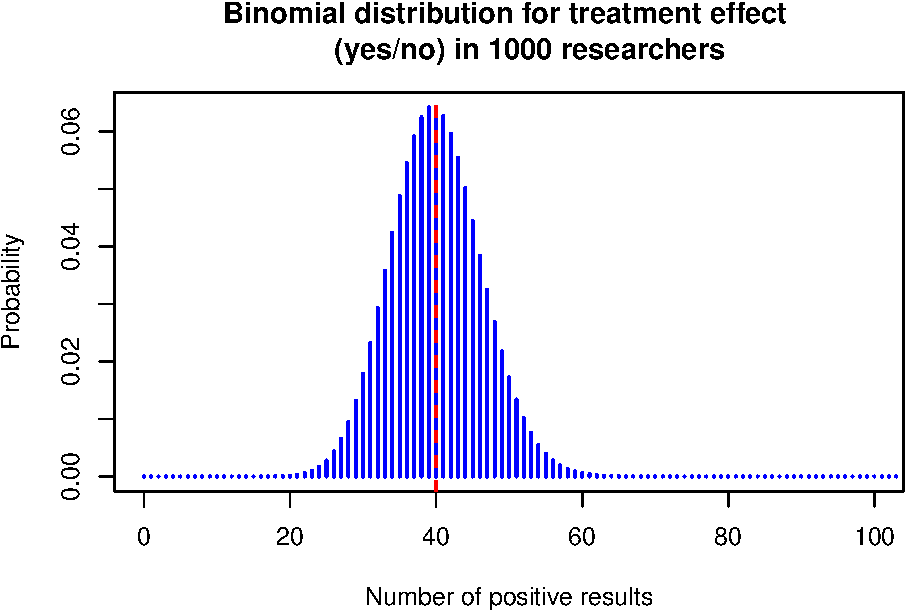
\includegraphics[keepaspectratio]{_main_files/figure-latex/unnamed-chunk-7-1.pdf}}

Note, this form of distribution looks like a bell curve, aka a \href{https://en.wikipedia.org/wiki/Normal_distribution}{normal distribution},
probably the most important distribution in statistics. One can \href{https://www.m-hikari.com/imf/imf-2017/9-12-2017/p/baguiIMF9-12-2017.pdf}{show formally} that the binomial distribution converges to the normal distribution under certain conditions.
So, if we would only have one shot to predict the number of researches reporting a treatment effect under the assumption that no treatment exists, we would bet on 40.
This guess would also not be too bad considering the whole range (0 to 1000) since we can expect the number of successes above, let's say, 65 and below, let's say, 15 to be very unlikely.

\begin{Shaded}
\begin{Highlighting}[]
\FunctionTok{sum}\NormalTok{(}\FunctionTok{dbinom}\NormalTok{(}\DecValTok{0}\SpecialCharTok{:}\DecValTok{14}\NormalTok{, }\AttributeTok{size =} \DecValTok{1000}\NormalTok{, }\AttributeTok{prob =} \FloatTok{0.04}\NormalTok{)) }\CommentTok{\# prob of 14 or less}
\end{Highlighting}
\end{Shaded}

\begin{verbatim}
## [1] 1.384829e-06
\end{verbatim}

\begin{Shaded}
\begin{Highlighting}[]
\FunctionTok{sum}\NormalTok{(}\FunctionTok{dbinom}\NormalTok{(}\DecValTok{66}\SpecialCharTok{:}\DecValTok{1000}\NormalTok{, }\AttributeTok{size =} \DecValTok{1000}\NormalTok{, }\AttributeTok{prob =} \FloatTok{0.04}\NormalTok{)) }\CommentTok{\# prob of 66 or more}
\end{Highlighting}
\end{Shaded}

\begin{verbatim}
## [1] 7.160623e-05
\end{verbatim}

\begin{Shaded}
\begin{Highlighting}[]
\FunctionTok{sum}\NormalTok{(}\FunctionTok{dbinom}\NormalTok{(}\DecValTok{15}\SpecialCharTok{:}\DecValTok{65}\NormalTok{, }\AttributeTok{size =} \DecValTok{1000}\NormalTok{, }\AttributeTok{prob =} \FloatTok{0.04}\NormalTok{)) }\CommentTok{\# prob of 15 to 65}
\end{Highlighting}
\end{Shaded}

\begin{verbatim}
## [1] 0.999927
\end{verbatim}

\textbf{The second question} asked about observing 137 positively reporting researchers.
We can calculate the probability of observing 137 or more positive results using the \href{https://en.wikipedia.org/wiki/Binomial_distribution}{binomial distribution}
(plug into the formula):
\(\mathbb{P}(\text{observing 137 or more}) = \sum_{i=137}^{1000} \binom{1000}{i}0.04^i (1-0.04)^{1000-i}\):

\begin{Shaded}
\begin{Highlighting}[]
\CommentTok{\# Calculate the probability of observing 137 or more positive results}
\CommentTok{\# (using the complement rule)}
\DecValTok{1} \SpecialCharTok{{-}} \FunctionTok{sum}\NormalTok{(}\FunctionTok{dbinom}\NormalTok{(}\DecValTok{0}\SpecialCharTok{:}\DecValTok{136}\NormalTok{, }\AttributeTok{size =} \DecValTok{1000}\NormalTok{, }\AttributeTok{prob =} \FloatTok{0.04}\NormalTok{))}
\end{Highlighting}
\end{Shaded}

\begin{verbatim}
## [1] 5.551115e-16
\end{verbatim}

\begin{Shaded}
\begin{Highlighting}[]
\CommentTok{\# Compare to winning the Swiss lottery}
\NormalTok{(}\DecValTok{1} \SpecialCharTok{/} \DecValTok{31474716}\NormalTok{) }\SpecialCharTok{/}\NormalTok{ (}\DecValTok{1} \SpecialCharTok{{-}} \FunctionTok{sum}\NormalTok{(}\FunctionTok{dbinom}\NormalTok{(}\DecValTok{0}\SpecialCharTok{:}\DecValTok{136}\NormalTok{, }\AttributeTok{size =} \DecValTok{1000}\NormalTok{, }\AttributeTok{prob =} \FloatTok{0.04}\NormalTok{)))}
\end{Highlighting}
\end{Shaded}

\begin{verbatim}
## [1] 57234507
\end{verbatim}

57 million times less likely than winning the Swiss lottery. If this event would happen, we would probably reject the assumption that the therapy is not working at all.

In the calculation above, we used the \href{https://en.wikipedia.org/wiki/Complement_(set_theory)}{complement rule} to calculate the probability of
observing 137 or more positive results: \(1 - \mathbb{P}(\text{observing 136 or less})\).

In general, for an event \(A\):

\[\mathbb{P}(A^C) = 1 - \mathbb{P}(A),\]

where \(A^C\) comprises all elementary events that are not in \(A\). In our case, the compliment of observing 136 or less is observing 137 or more and vice versa:
\(\mathbb{P}(0, \dots, 136) = 1 - \mathbb{P}((0, \dots, 136)^C) = 1 - \mathbb{P}(137, \dots, 1000)\).

\textbf{The third question} asked about the expected number of positive results if the therapy is working in 12\% of the patients.
As you can probably guess by now: We would guess \(1000 \times 0.12 = 120\) positive results.
This is the so-called \textbf{\href{https://en.wikipedia.org/wiki/Expected_value}{expected value}} \(\mathbb{E}(X)\) of the \href{https://en.wikipedia.org/wiki/Binomial_distribution}{binomial distribution}.
It is not always the maximum probability (the so-called \href{https://en.wikipedia.org/wiki/Mode_(statistics)}{mode}) of the distribution though:
Consider a binomial distribution \(\text{Bin}(10, 0.77)\):

\begin{itemize}
\tightlist
\item
  The \textbf{mean} is \(\mathbb{E}(X) = 10 \times 0.77 = 7.7\). This number is not an integer and we can therefore not calculate the density at this point.
\item
  The \textbf{\href{https://en.wikipedia.org/wiki/Mode_(statistics)}{mode}} is 8.
\end{itemize}

\textbf{The fourth question} asked about the problem of writing a press release stating that 47 out of 50 studies showed a treatment effect.
Well, this would be scientific fraud and a case of \href{https://en.wikipedia.org/wiki/Survivorship_bias\#:~:text=Survivorship\%20bias\%20or\%20survival\%20bias,conclusions\%20because\%20of\%20incomplete\%20data.}{survivorship bias}.
You only look at the studies that showed a treatment effect and ignore the ones that did not or you restrict the number of studies to a certain number lower than the true number.
This is also relevant in \href{https://www.investopedia.com/terms/s/survivorship-bias-risk.asp\#:~:text=This\%20risk\%20arises\%20from\%20focusing,or\%20removed\%20from\%20performance\%20data.}{finance}.
You may want to read this excellent \href{https://journals.plos.org/plosmedicine/article?id=10.1371/journal.pmed.0020124}{article} by John Ioannidis for a humbling big-picture of how relevant published results can be.

\textbf{The fifth question} asked about the problem of \href{https://en.wikipedia.org/wiki/Multiple_comparisons_problem}{multiple testing}.
If you test many hypotheses, you will find some ``significant'' results by chance alone.
One could also call the practice of testing many hypotheses to find ``significant'' ones \href{https://en.wikipedia.org/wiki/Data_dredging}{p-hacking}.
This should be absolutely avoided. Unfornately, it is still common practice in many fields. Often it happens unconsciously.
Example: If you test 100 hypotheses simultaneously at a significance level of 4\%, you would expect 4 ``significant'' results by chance alone.
If you report those 4 results as legitimate finding, you are p-hacking. When reading a scientific article, watch out for large amounts of p-values and
their (over-)interpretation as ``significant'' (relevant) or ``non-significant'' (not relevant).
This \href{https://www.tandfonline.com/doi/full/10.1080/00031305.2019.1583913}{article} is recommendable to get away from a too strict dichotomous interpretation of research results.

\textbf{The sixth question} asked about the variation of positive results between large research departments. This demands the very important concept of \href{https://en.wikipedia.org/wiki/Variance}{variance}:
The expected quadratic deviation from the mean: \(\mathbb{V}ar(X) = \mathbb{E} \{ (\mathbb{E}(X) - X)^2 \}\). In simple terms:
How much does the number of positive results vary around the mean of 40 on average?
See also \hyperref[exercise5]{Exercise 5}. Maybe this \href{https://www.youtube.com/watch?v=SzZ6GpcfoQY}{video} helps as well.

\subsection{Addition of probabilities}\label{addition_of_probabilities}

\hyperref[axioms_of_probability_theory]{Above} in axiom 3, we stated that the probability of the union of pairwise disjoint events is the sum of the
probabilities of the individual events.
What if the events are not disjoint? For simplicity, let's consider only 2 researchers (doing 2 parallel experiments) and define event \(A_1\) as ``researcher 1 finds an effect'' and
\(A_2\) as ``researcher 2 finds an effect''.
What is the probability that at least one of the researchers finds an effect?
Our event space
\(\Omega = \{ (R1pos, R2pos), (R1pos, R2neg), (R1neg, R2pos), (R1neg, R2neg) \}.\)

\(\sum_{\omega_i} \mathbb{P}(\omega_i) = 0.04^2 + 0.04 \times 0.96 + 0.96 \times 0.04 + 0.96^2 = 1\)

\(A_1 \cup A_2 = \{ (R1pos, R2pos), (R1pos, R2neg), (R1neg, R2pos)\}\)

\(A_1 = \{ (R1pos, R2pos), (R1pos, R2neg)\}\)

\(A_2 = \{ (R1pos, R2pos), (R1neg, R2pos)\}\)

\(\mathbb{P}(A_1) = 0.04^2 + 0.04 \times 0.96\) (First researcher finds an effect or both find an effect)

\(\mathbb{P}(A_2) = 0.04^2 + 0.96 \times 0.04\) (Second researcher finds an effect or both find an effect)

In, general, we can write the \href{https://en.wikipedia.org/wiki/Probability\#Not_(necessarily)_mutually_exclusive_events}{probability of the union of two events} as:
\(\mathbb{P}(A_1 \cup A_2) = \mathbb{P}(A_1) + \mathbb{P}(A_2) - \mathbb{P}(A_1 \cap A_2)\)

Put in the values:
\(0.04^2 + 0.04 \times 0.96 +\)
\(0.04^2 + 0.96 \times 0.04 - 0.04^2=\)
\(0.04^2 + 0.04 \times 0.96 + 0.96 \times 0.04. = 0.0784\).

Or simpler with the \textbf{complement rule}:

\(\mathbb{P}(A_1 \cup A_2) = 1 - \mathbb{P}(\text{neither }A_1 \text{ nor }A_2) = 1-0.96^2 = 0.0784\).

See also \hyperref[exercise6]{Exercise 6}.

\pandocbounded{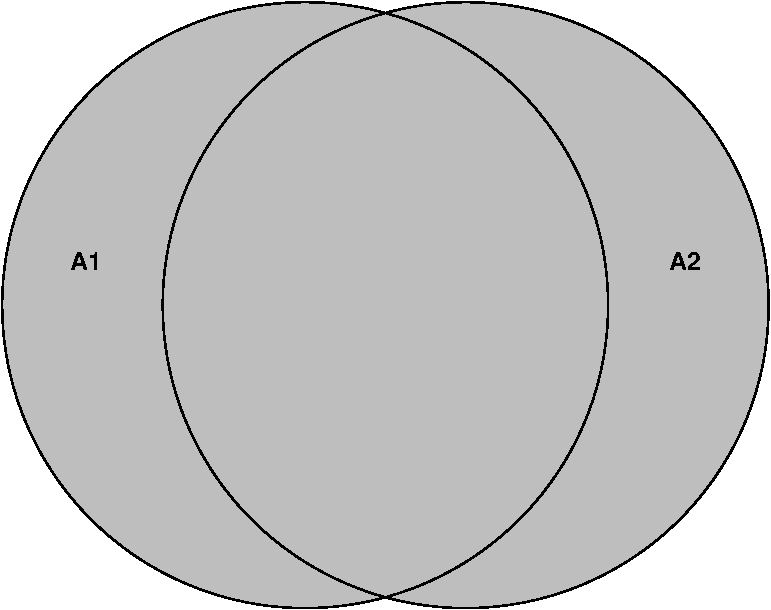
\includegraphics[keepaspectratio]{_main_files/figure-latex/unnamed-chunk-10-1.pdf}}

Here is another helpful depiction of the situation:

\pandocbounded{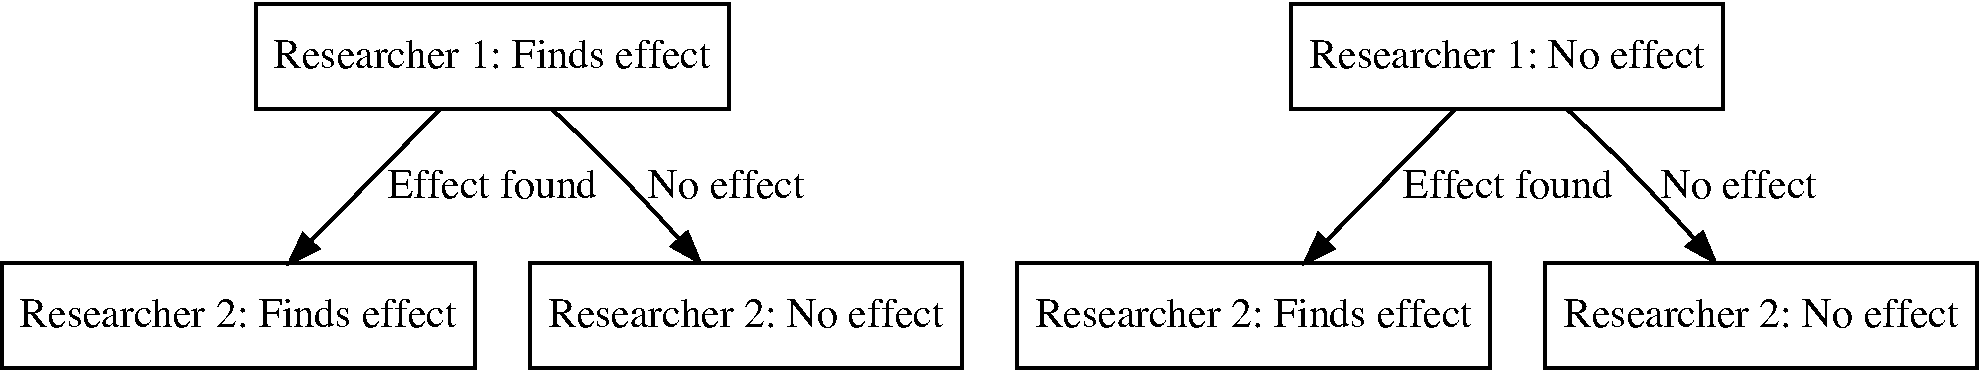
\includegraphics[keepaspectratio]{_main_files/figure-latex/unnamed-chunk-11-1.pdf}}

So, the probability of at least one researcher finding an effect is the sum of the probabilities of the individual researchers finding an effect minus
the probability of both finding an effect, which is the same as that both or exactly one of them finds an effect.

We can also visualize the 4 disjoint elementary events
\[\Omega = \{ (R1pos, R2pos), (R1pos, R2neg), (R1neg, R2pos), (R1neg, R2neg) \}\]
in a \href{https://en.wikipedia.org/wiki/Venn_diagram}{Venn diagram}. The probabilites of these
4 events in the event space \(\Omega\) must add up to 1 since they are disjoint and one of them has to happen. There is no ``room'' left.

\pandocbounded{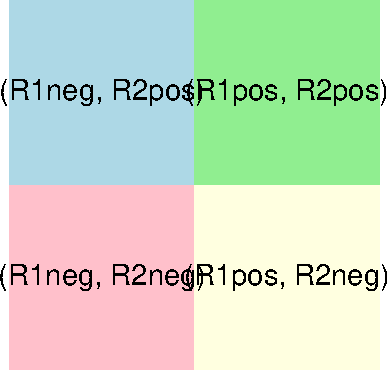
\includegraphics[keepaspectratio]{_main_files/figure-latex/unnamed-chunk-12-1.pdf}}

\subsection{Probabilities for health science}\label{probabilities_for_health_sciences}

We have learned a lot so far: The axioms of probability theory, the difference between independence and disjointness, and the addition of probabilities.

\textbf{How does probability theory fit into the big picture of statistics for health sciences?}

In many health-related studies, we want to perform one or more of the following tasks:

\begin{itemize}
\tightlist
\item
  Estimate proportions (e.g., the proportion of patients with lower back pain. How big is the problem from a public health perspective?),
\item
  Test hypotheses (e.g., whether a new therapy is superior to the standard therapy. How sure can we be that the new therapy is better?
  What is the probability that the treatment effect is between x and y points on some scale?),
\item
  Estimate therapy effects (e.g., the effect of a new therapy on pain reduction:
  How many points does the pain decrease? How is the pain reduction distributed?
  Are there outliers and why? Are there participants that to not benefit from the therapy?)
\end{itemize}

In all such cases, probability theory is the established tool to answer questions that are afflicted with uncertainty. Would there be no variation in results/effects,
we would probably argue differently. In our world, probability theory is the tool to \textbf{quantify uncertainty}.

We can always ask ourselves: Where is this entity (proportion, effect, etc.) with which frequency/probability?

\subsection{Discrete vs.~continuous probability distributions}\label{discrete_vs_continuous_probability_distributions}

As one of the most prominent examples of a discrete distribution, we have already seen
the \href{https://en.wikipedia.org/wiki/Binomial_distribution}{binomial distribution} in our 1000-researcher-experiment.
A special case of it is the \href{https://en.wikipedia.org/wiki/Bernoulli_distribution}{Bernoulli distribution},
where you only throw the coin once or let one researcher conduct the experiment.

As an example of a continuous distribution we have mentioned the \href{https://en.wikipedia.org/wiki/Normal_distribution}{normal distribution} above.
It is the most important distribution in statistics for reasons that become increasingly clear as we go along.
One of them is the \href{https://en.wikipedia.org/wiki/Central_limit_theorem}{central limit theorem} which we have already mentioned in the
introduction slides. Feel free to watch this \href{https://www.youtube.com/watch?v=zeJD6dqJ5lo&t=28s&ab_channel=3Blue1Brown}{video}.
The theorem states that, under appropriate conditions, the distribution of a normalized version of the sample
mean (\(\bar{X} = \sum_{i=1}^{n} X_i\)) converges to a standard normal distribution.
By this theorem, we can link \textbf{any} distribution to the normal distribution.

Discrete or continuous, the \textbf{goal} is the same: We want to now \textbf{where} the realization of my \textbf{random variable} lands \textbf{with what probability}
when I do the experiment?
How often will I get heads?

\begin{itemize}
\item
  How often will the researcher find an effect?
\item
  With what probability will I get a pain-score reduction of at least 1 point in this patient in front of me given his/her
  characteristics and history?
\item
  When looking at ZHAW students, female, soccer lovers, what kind of hourly intense sports activity can I expect and does that differ to other groups?
\end{itemize}

For us, the following definitions should suffice.

\subsubsection{Discrete probability distrubtions are used when we can count the outcomes, which includes infinitely many.}\label{discrete_probability_distributions}

Some examples of \href{https://en.wikipedia.org/wiki/Probability_distribution\#Discrete_probability_distribution}{discrete probability distributions} are:
- \textbf{\href{https://en.wikipedia.org/wiki/Bernoulli_distribution}{Bernoulli distribution}}: A single trial with two outcomes (e.g., find an effect or do not find an effect).
- \textbf{\href{https://en.wikipedia.org/wiki/Binomial_distribution}{Binomial distribution}}: The number of successes in a fixed number of trials (e.g., the number of false effects found among 1000 researchers).
- \textbf{\href{https://en.wikipedia.org/wiki/Poisson_distribution}{Poisson distribution}}: The number of events in a fixed interval of time or space.
- \textbf{\href{https://en.wikipedia.org/wiki/Geometric_distribution}{Geometric distribution}}: The number of trials until the first success. This number has no upper limit.

We always assign probabilites to the countable outcomes of these distributions, like in the example of the binomial distribution when
we throw the dice 20 times and are interested in the number of 3s:

\begin{Shaded}
\begin{Highlighting}[]
\CommentTok{\# Define parameters for the binomial distribution}
\NormalTok{x\_values }\OtherTok{\textless{}{-}} \DecValTok{0}\SpecialCharTok{:}\DecValTok{20}
\NormalTok{probabilities }\OtherTok{\textless{}{-}} \FunctionTok{dbinom}\NormalTok{(x\_values, }\AttributeTok{size =} \DecValTok{20}\NormalTok{, }\AttributeTok{prob =} \DecValTok{1} \SpecialCharTok{/} \DecValTok{6}\NormalTok{)}

\CommentTok{\# Plot the binomial distribution with styling}
\FunctionTok{plot}\NormalTok{(x\_values, probabilities, }\AttributeTok{type =} \StringTok{"h"}\NormalTok{, }\AttributeTok{lwd =} \DecValTok{2}\NormalTok{, }\AttributeTok{col =} \StringTok{"blue"}\NormalTok{,}
     \AttributeTok{xlab =} \StringTok{"X"}\NormalTok{, }\AttributeTok{ylab =} \StringTok{"Probability"}\NormalTok{,}
     \AttributeTok{main =} \StringTok{"Binomial Probability Distribution (n = 20, p = 1/6)"}\NormalTok{)}

\CommentTok{\# Add points for clarity}
\FunctionTok{points}\NormalTok{(x\_values, probabilities, }\AttributeTok{pch =} \DecValTok{19}\NormalTok{, }\AttributeTok{col =} \StringTok{"red"}\NormalTok{)}
\end{Highlighting}
\end{Shaded}

\pandocbounded{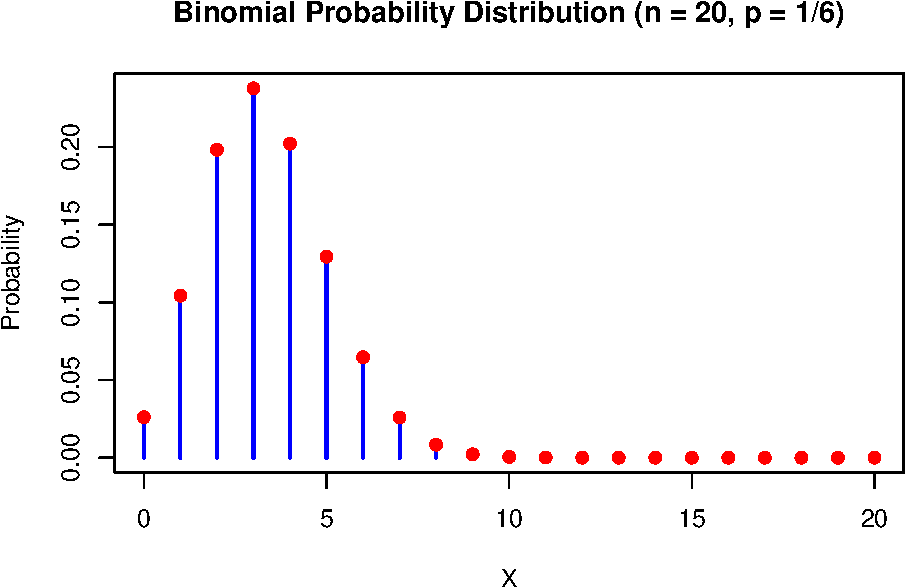
\includegraphics[keepaspectratio]{_main_files/figure-latex/unnamed-chunk-13-1.pdf}}

Each outcome has a probability \(>0\) assigned to it. The sum of all probabilities is 1: \(\sum_{i \in \text{Possible outcomes}} \mathbb{P}(X=i) = 1\).
For every event, we just add the probabilities of the elementary outcomes that are in the event:

\(\mathbb{P}(X \in (3,8,9,14)) = \mathbb{P}(X = 3) + \mathbb{P}(X = 8) + \mathbb{P}(X = 9) + \mathbb{P}(X = 14)\).
This principle is true for all discrete probability distributions. Rather simple and elegant:

\[\sum_{i} \mathbb{P}(X = x_i) = 1,\]

where \(X\) ist the random variable (which takes values \(x_i\) when the random experiment is conducted) and \(x_i\) are the possible outcomes of \(X\).

We could \textbf{invent our own discrete probability distribution} instantly (see also \hyperref[exercise8]{Exercise 8}), we'll call it the MSc-ZHAW-distribution:

Let \(X \in \mathbb{Z}\). Every whole number gets the following probability:
\(\mathbb{P}(X=0) = 0.1\) and for \(x_i \neq 0\): \(\mathbb{P}(X = x_i) = 0.2^{|x_i|}\).
The sum of all probabilities is: \(\sum_{x_i \in \mathbb{Z}} \mathbb{P}(X=x_i) = \mathbb{P}(X=0) + 2 \cdot \sum_{i \in \mathbb{N}} 0.2^i =
0.1 + 2 \cdot \frac{0.2}{1-0.2} = 0.6\). Hence, we need to divide every probability by 0.6 to get in sum 1.
The final definition is then:

\(\mathbb{P}(X=0) = \frac{1}{6}\) and for \(x_i \neq 0\): \(\mathbb{P}(X = x_i) = \frac{5}{3} 0.2^{|x_i|}\).

\begin{Shaded}
\begin{Highlighting}[]
\CommentTok{\# Define the probability function}
\NormalTok{P }\OtherTok{\textless{}{-}} \ControlFlowTok{function}\NormalTok{(X) \{}
  \ControlFlowTok{if}\NormalTok{ (X }\SpecialCharTok{==} \DecValTok{0}\NormalTok{) \{}
    \FunctionTok{return}\NormalTok{(}\DecValTok{1} \SpecialCharTok{/} \DecValTok{6}\NormalTok{)}
\NormalTok{  \} }\ControlFlowTok{else}\NormalTok{ \{}
    \FunctionTok{return}\NormalTok{((}\DecValTok{5} \SpecialCharTok{/} \DecValTok{3}\NormalTok{) }\SpecialCharTok{*}\NormalTok{ (}\FloatTok{0.2}\SpecialCharTok{\^{}}\FunctionTok{abs}\NormalTok{(X)))}
\NormalTok{  \}}
\NormalTok{\}}

\CommentTok{\# Create a sequence of X values from {-}10 to 10}
\NormalTok{X\_values }\OtherTok{\textless{}{-}} \SpecialCharTok{{-}}\DecValTok{10}\SpecialCharTok{:}\DecValTok{10}

\CommentTok{\# Compute the probabilities for each X value}
\NormalTok{probabilities }\OtherTok{\textless{}{-}} \FunctionTok{sapply}\NormalTok{(X\_values, P)}

\CommentTok{\# Plot the probabilities}
\FunctionTok{plot}\NormalTok{(X\_values, probabilities, }\AttributeTok{type =} \StringTok{"h"}\NormalTok{, }\AttributeTok{lwd =} \DecValTok{2}\NormalTok{, }\AttributeTok{col =} \StringTok{"blue"}\NormalTok{,}
     \AttributeTok{xlab =} \StringTok{"X"}\NormalTok{, }\AttributeTok{ylab =} \StringTok{"Probability"}\NormalTok{,}
     \AttributeTok{main =} \StringTok{"MSc{-}ZHAW Probability Distribution of X from {-}10 to 10"}\NormalTok{)}

\CommentTok{\# Add points for clarity}
\FunctionTok{points}\NormalTok{(X\_values, probabilities, }\AttributeTok{pch =} \DecValTok{19}\NormalTok{, }\AttributeTok{col =} \StringTok{"red"}\NormalTok{)}
\end{Highlighting}
\end{Shaded}

\pandocbounded{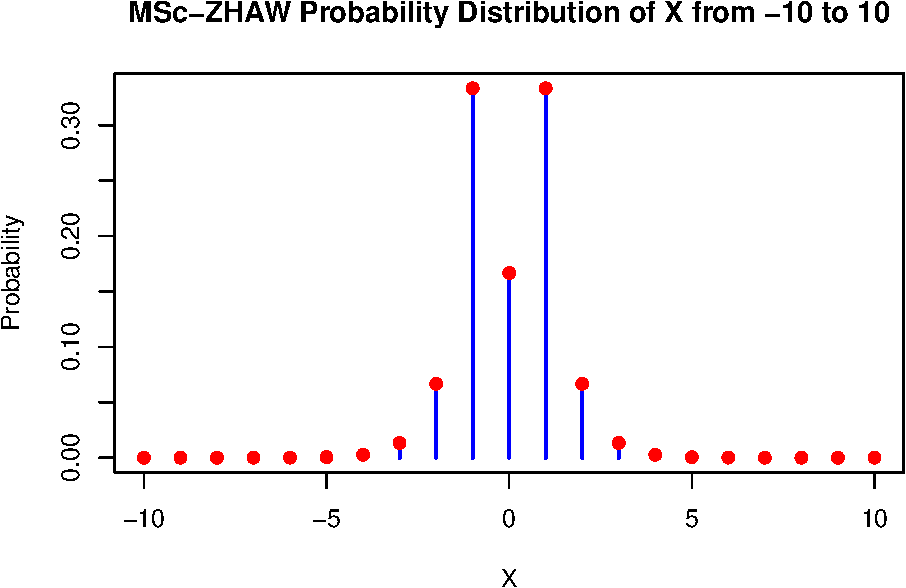
\includegraphics[keepaspectratio]{_main_files/figure-latex/unnamed-chunk-14-1.pdf}}

\begin{Shaded}
\begin{Highlighting}[]
\CommentTok{\# Check if it sums to 1 (approximately):}
\NormalTok{x\_values }\OtherTok{\textless{}{-}} \SpecialCharTok{{-}}\DecValTok{1000}\SpecialCharTok{:}\DecValTok{1000}
\FunctionTok{sum}\NormalTok{(}\FunctionTok{sapply}\NormalTok{(x\_values, P))}
\end{Highlighting}
\end{Shaded}

\begin{verbatim}
## [1] 1
\end{verbatim}

Deviations from zero (\(\pm 1\)) are highly likely with this distribution. The probability of \(X=0\) is also rather high with \(\frac{1}{6}\).
Larger deviations from zero are less likely and go exponentially towards zero (very fast). So we would expect almost never to see values outside
of \(\pm 10\). This does of course not mean that we will never see them. Do the experiment often enough and you will seen them with
probability 1 (see \hyperref[exercise10]{Exercise 10}).

\begin{Shaded}
\begin{Highlighting}[]
\NormalTok{x\_values }\OtherTok{\textless{}{-}} \FunctionTok{setdiff}\NormalTok{(}\SpecialCharTok{{-}}\DecValTok{1000}\SpecialCharTok{:}\DecValTok{1000}\NormalTok{, }\SpecialCharTok{{-}}\DecValTok{10}\SpecialCharTok{:}\DecValTok{10}\NormalTok{) }\CommentTok{\# exclude values from {-}10 to 10}
\FunctionTok{sum}\NormalTok{(}\FunctionTok{sapply}\NormalTok{(x\_values, P))}
\end{Highlighting}
\end{Shaded}

\begin{verbatim}
## [1] 8.533333e-08
\end{verbatim}

\textbf{Expectation \(\mathbb{E}(X)\) of a discrete random variable}: The expectation of a discrete random variable \(X\) is defined as:

\[\mu = \mathbb{E}(X) = \sum x_i \cdot \mathbb{P}(X = x_i),\]

a weighted sum of possible values \(x_i\) with their respsective probabilities \(\mathbb{P}(X = x_i)\).

The term ``expectation'' is probably somewhat misleading. It is not necessarily the value we ``expect to see'' when we do the experiment. For instance,
the expected value of a Bernoulli distribution is: \(\mu = \mathbb{E}(X) = 0 \cdot (1-p) + 1 \cdot p = p\), which could be \(0.5\). The individual outcomes are \(0\) and \(1\),
and not \(0.5\). But \(0.5\) would be the mean of many experiments.

The expectation can be interpreted as the \href{https://mathcenter.oxford.emory.edu/site/math117/expectedValueAndCenterOfMass/}{center of mass}
of the distribution. It is the value that the distribution ``balances'' around.

Maybe this \href{https://www.youtube.com/watch?v=KLs_7b7SKi4}{video} helps too.

The cool thing is that we can learn the true (but unknown) expectation of a distribution by the sample mean. The more samples we collect, the closer we will be.
This is (roughly) the statement of the \href{https://en.wikipedia.org/wiki/Law_of_large_numbers}{law of large numbers}:

\[\bar{X}_n \rightarrow \mu = \mathbb{E}(X) \quad \text{as} \quad n \rightarrow \infty.\]

See \href{https://github.com/jdegenfellner/ZHAW_Teaching/blob/main/Law_of_Large_Numbers_Dice_animation.R}{here} for an animated example of this law.

\textbf{Remember}: The sample mean \(\bar{x} = \frac{1}{n} \sum_{i=1}^n x_i\) is a (really good) estimator for the expectation \(\mu = \mathbb{E}(X)\) of a distribution.
This is true for discrete and continuous distributions.

The \textbf{variance of a discrete random variable} is defined as:

\[\mathbb{V}ar(X) = \mathbb{E} \{ (\mathbb{E}(X) - X)^2 \} = \sum_i (\mathbb{E}(X) - x_i)^2 \mathbb{P}(X = x_i),\]

the expected squared deviation from the mean. It is a measure of how much the values of the random variable differ from the mean.

\textbf{Remember}: The sample variance \(s^2 = \frac{1}{n-1} \sum_{i=1}^n (x_i - \bar{x})^2\) is an estimator for the variance \(\mathbb{V}ar(X)\) of a distribution.
This is true for discrete and continuous distributions.

A more natural interpretation of variability is the \textbf{standard deviation}:

\[\sigma = \sqrt{\mathbb{V}ar(X)},\]

since it's on the same scale as X.

\subsubsection{Continuous probability distributions are used when we cannot count the outcomes.}\label{continuous_probability_distributions}

The most famous continuous probability distribution is the
\href{https://en.wikipedia.org/wiki/Normal_distribution}{normal distribution}.
This \href{https://www.youtube.com/watch?v=k5sbE1_MDwU&ab_channel=VeryNormal}{video}
about probability distributions in general might be helpful.

\begin{Shaded}
\begin{Highlighting}[]
\CommentTok{\# Load necessary library}
\ControlFlowTok{if}\NormalTok{ (}\SpecialCharTok{!}\FunctionTok{require}\NormalTok{(pacman)) }\FunctionTok{install.packages}\NormalTok{(}\StringTok{"pacman"}\NormalTok{)}
\end{Highlighting}
\end{Shaded}

\begin{verbatim}
## Loading required package: pacman
\end{verbatim}

\begin{Shaded}
\begin{Highlighting}[]
\NormalTok{pacman}\SpecialCharTok{::}\FunctionTok{p\_load}\NormalTok{(ggplot2) }\CommentTok{\# Installs and loads the package at the same time}

\CommentTok{\# Define parameters for the normal distribution}
\NormalTok{mu }\OtherTok{\textless{}{-}} \DecValTok{0}    \CommentTok{\# Mean}
\NormalTok{sigma }\OtherTok{\textless{}{-}} \DecValTok{1} \CommentTok{\# Standard deviation}

\CommentTok{\# Define the limits for the area to be shaded}
\NormalTok{a }\OtherTok{\textless{}{-}} \SpecialCharTok{{-}}\DecValTok{2}  \CommentTok{\# Lower bound}
\NormalTok{b }\OtherTok{\textless{}{-}} \SpecialCharTok{{-}}\DecValTok{1}   \CommentTok{\# Upper bound}

\CommentTok{\# Create a sequence of x values to evaluate the PDF}
\NormalTok{x\_vals }\OtherTok{\textless{}{-}} \FunctionTok{seq}\NormalTok{(mu }\SpecialCharTok{{-}} \DecValTok{4} \SpecialCharTok{*}\NormalTok{ sigma, mu }\SpecialCharTok{+} \DecValTok{4} \SpecialCharTok{*}\NormalTok{ sigma, }\AttributeTok{length.out =} \DecValTok{1000}\NormalTok{)}

\CommentTok{\# Compute the corresponding density values using dnorm}
\NormalTok{y\_vals }\OtherTok{\textless{}{-}} \FunctionTok{dnorm}\NormalTok{(x\_vals, }\AttributeTok{mean =}\NormalTok{ mu, }\AttributeTok{sd =}\NormalTok{ sigma)}

\CommentTok{\# Create a data frame for plotting}
\NormalTok{df }\OtherTok{\textless{}{-}} \FunctionTok{data.frame}\NormalTok{(}\AttributeTok{x =}\NormalTok{ x\_vals, }\AttributeTok{density =}\NormalTok{ y\_vals)}

\CommentTok{\# Create a subset of the data for shading the area between a and b}
\NormalTok{df\_shaded }\OtherTok{\textless{}{-}}\NormalTok{ df[df}\SpecialCharTok{$}\NormalTok{x }\SpecialCharTok{\textgreater{}=}\NormalTok{ a }\SpecialCharTok{\&}\NormalTok{ df}\SpecialCharTok{$}\NormalTok{x }\SpecialCharTok{\textless{}=}\NormalTok{ b, ]}

\CommentTok{\# Plot the normal density and shade the area between a and b}
\FunctionTok{ggplot}\NormalTok{(df, }\FunctionTok{aes}\NormalTok{(}\AttributeTok{x =}\NormalTok{ x, }\AttributeTok{y =}\NormalTok{ density)) }\SpecialCharTok{+}
  \FunctionTok{geom\_line}\NormalTok{(}\AttributeTok{color =} \StringTok{"blue"}\NormalTok{, }\AttributeTok{linewidth =} \DecValTok{1}\NormalTok{) }\SpecialCharTok{+}  \CommentTok{\# Use linewidth instead of size}
  \FunctionTok{geom\_ribbon}\NormalTok{(}\AttributeTok{data =}\NormalTok{ df\_shaded, }\FunctionTok{aes}\NormalTok{(}\AttributeTok{ymin =} \DecValTok{0}\NormalTok{, }\AttributeTok{ymax =}\NormalTok{ density),}
              \AttributeTok{fill =} \StringTok{"blue"}\NormalTok{, }\AttributeTok{alpha =} \FloatTok{0.3}\NormalTok{) }\SpecialCharTok{+}  \CommentTok{\# Shaded area}
  \FunctionTok{ggtitle}\NormalTok{(}\FunctionTok{paste}\NormalTok{(}\StringTok{"Standard Normal Distribution: }
\StringTok{  N("}\NormalTok{, mu, }\StringTok{", "}\NormalTok{, sigma}\SpecialCharTok{\^{}}\DecValTok{2}\NormalTok{, }\StringTok{")"}\NormalTok{, }\AttributeTok{sep =} \StringTok{""}\NormalTok{)) }\SpecialCharTok{+}
  \FunctionTok{xlab}\NormalTok{(}\StringTok{"X"}\NormalTok{) }\SpecialCharTok{+}
  \FunctionTok{ylab}\NormalTok{(}\StringTok{"Density"}\NormalTok{) }\SpecialCharTok{+}
  \FunctionTok{theme\_minimal}\NormalTok{() }\SpecialCharTok{+}
  \FunctionTok{geom\_vline}\NormalTok{(}\AttributeTok{xintercept =}\NormalTok{ mu, }\AttributeTok{color =} \StringTok{"red"}\NormalTok{, }\AttributeTok{linetype =} \StringTok{"dashed"}\NormalTok{) }\SpecialCharTok{+}
  \FunctionTok{annotate}\NormalTok{(}\StringTok{"text"}\NormalTok{, }\AttributeTok{x =}\NormalTok{ mu }\SpecialCharTok{+} \FloatTok{0.2}\NormalTok{, }\AttributeTok{y =} \FunctionTok{max}\NormalTok{(y\_vals) }\SpecialCharTok{/} \DecValTok{2}\NormalTok{,}
           \AttributeTok{label =} \FunctionTok{paste}\NormalTok{(}\StringTok{"E(X) ="}\NormalTok{, mu), }\AttributeTok{color =} \StringTok{"red"}\NormalTok{) }\SpecialCharTok{+}
  \FunctionTok{geom\_vline}\NormalTok{(}\AttributeTok{xintercept =}\NormalTok{ a, }\AttributeTok{color =} \StringTok{"black"}\NormalTok{, }\AttributeTok{linetype =} \StringTok{"dashed"}\NormalTok{) }\SpecialCharTok{+}
  \FunctionTok{geom\_vline}\NormalTok{(}\AttributeTok{xintercept =}\NormalTok{ b, }\AttributeTok{color =} \StringTok{"black"}\NormalTok{, }\AttributeTok{linetype =} \StringTok{"dashed"}\NormalTok{) }\SpecialCharTok{+}
  \FunctionTok{annotate}\NormalTok{(}\StringTok{"text"}\NormalTok{, }\AttributeTok{x =}\NormalTok{ a }\SpecialCharTok{{-}} \FloatTok{0.2}\NormalTok{, }\AttributeTok{y =} \FunctionTok{max}\NormalTok{(y\_vals) }\SpecialCharTok{/} \DecValTok{4}\NormalTok{,}
           \AttributeTok{label =} \FunctionTok{paste}\NormalTok{(}\StringTok{"a ="}\NormalTok{, a), }\AttributeTok{color =} \StringTok{"black"}\NormalTok{) }\SpecialCharTok{+}
  \FunctionTok{annotate}\NormalTok{(}\StringTok{"text"}\NormalTok{, }\AttributeTok{x =}\NormalTok{ b }\SpecialCharTok{+} \FloatTok{0.2}\NormalTok{, }\AttributeTok{y =} \FunctionTok{max}\NormalTok{(y\_vals) }\SpecialCharTok{/} \DecValTok{4}\NormalTok{,}
           \AttributeTok{label =} \FunctionTok{paste}\NormalTok{(}\StringTok{"b ="}\NormalTok{, b), }\AttributeTok{color =} \StringTok{"black"}\NormalTok{) }\SpecialCharTok{+}
  \FunctionTok{theme}\NormalTok{(}\AttributeTok{plot.title =} \FunctionTok{element\_text}\NormalTok{(}\AttributeTok{hjust =} \FloatTok{0.5}\NormalTok{))}
\end{Highlighting}
\end{Shaded}

\pandocbounded{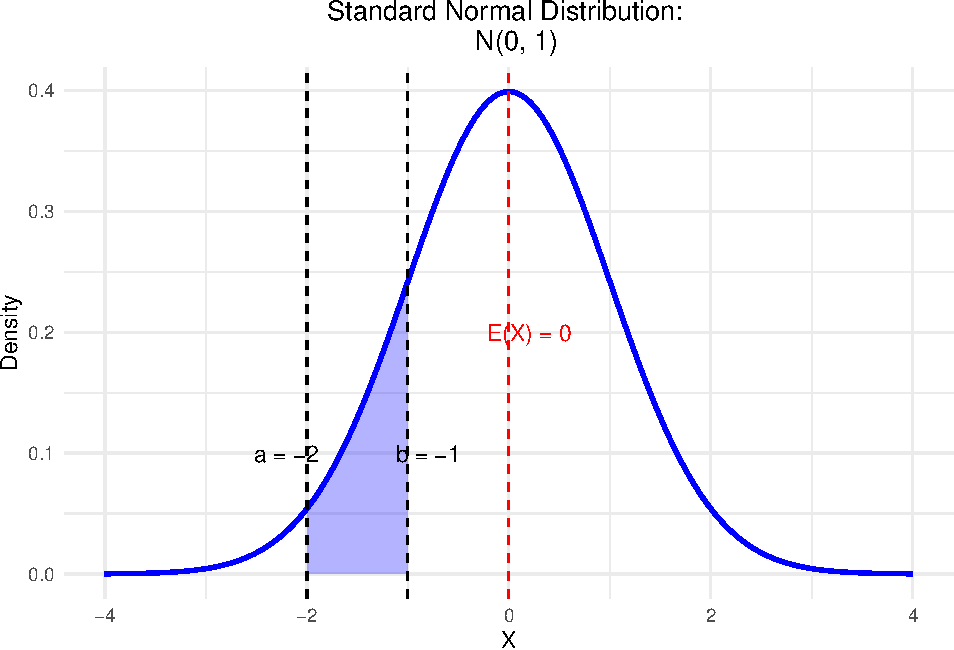
\includegraphics[keepaspectratio]{_main_files/figure-latex/unnamed-chunk-16-1.pdf}}

Here, like in any other ``nice'' continuous distribution, the area under the curve is 1:

\[\int_{-\infty}^{\infty} f(x) dx = 1.\]

The probability of a single point is zero (\(\mathbb{P}(\{ x_i \}) = 0\)).
In any continuous distribution, we use the area under the curve to calculate probabilities. The probability of \(X\) being between \(a\) and \(b\) is the area under the curve (blue shade) between \(a\) and \(b\):
\(\mathbb{P}(X \in (a,b))\). Note that the area over a single point would be zero and therefore the probability of a single point is zero.

The graph above is called a \href{https://en.wikipedia.org/wiki/Probability_density_function}{probability density function} (PDF).
Over every point, we express the probability by the height of the curve.
See \hyperref[exercise3_descriptive_stats]{exercise 3} in the next chapter for a practical example for what we will use this in research.

\textbf{Expectation \(\mathbb{E}(X)\) of a continuous random variable}: The expectation of a continuous random variable \(X\) is defined as:

\[\mu = \mathbb{E}(X) = \int x \cdot f(x) dx,\]

where \(x\) are the possible values of \(X\) and \(f(x)\) is the probability density function of \(X\).

\textbf{Variance of a continuous random variable}: The variance of a continuous random variable \(X\) is defined as:

\[\mathbb{V}ar(X) = \mathbb{E} \{ (\mathbb{E}(X) - X)^2 \} = \int (\mathbb{E}(X) - x)^2 f(x) dx.\]

A more natural interpretation of variability is the \textbf{standard deviation}:

\[\sigma = \sqrt{\mathbb{V}ar(X)},\]

since it's on the same scale as X.

Example: Normally distributed Ages of ZHAW students: \(\mu = 24\), \(\sigma = 3\). For the normal distribution,
this means that approx. 68\% of the students are between \((24-3=)21\) and \((24+3=)27\) years old.

\subsection{Examples of prominent probability distributions used in health sciences}\label{prominent_probability_distributions_in_health_sciences}

The first 2 are absolutely essential.

\begin{itemize}
\item
  The most important one is, as mentioned above, the \href{https://en.wikipedia.org/wiki/Normal_distribution}{normal distribution}.
  It is often used to model the distribution of many variables in health sciences, e.g., blood pressure, weight, height, etc.
  Normality is also a common assumption in many statistical tests and models. This is the reason why you will find many statements like
  ``we have checked normality using the shapiro-wilk test'' (Which I would not recommend) in scientific articles.
  Normal distribution theory is very aesthetic and one is sometimes lead to believe that this is the normal state of nature, which is
  not the case. See also the \href{https://en.wikipedia.org/wiki/Normal_distribution\#History}{history} of the normal distribution.
  A common use of the normal distribution is in \href{https://en.wikipedia.org/wiki/Linear_regression}{linear regression},
  where the errors and the conditional distribution of the modeled variable in the model are assumed to be normally distributed.
  We will deal with this in QM2.
\item
  The \href{https://en.wikipedia.org/wiki/Binomial_distribution}{binomial distribution} (\(X \sim B(n, p)\)) is used to model the number of successes in a fixed number of trials.
  For example, the number of patients that respond to a therapy in a fixed number of patients.
  A special case of it is the \href{https://en.wikipedia.org/wiki/Bernoulli_distribution}{Bernoulli distribution},
  which is used to model a single trial with two outcomes (throw the coin once; \(X \sim B(1,p)\)).
\item
  \href{https://en.wikipedia.org/wiki/Logistic_distribution}{Logistic Distribution}. Underpins logistic regression models,
  which are used to predict binary outcomes (e.g., the presence or absence of a disease).
\item
  \href{https://en.wikipedia.org/wiki/Poisson_distribution}{Poisson distribution}. Used to model the number of events in a fixed interval of time or space.
  For example, the number of patients arriving at an emergency department in a fixed time interval.
\item
  \href{https://en.wikipedia.org/wiki/Exponential_distribution}{Exponential distribution}.
  For instance used in survival analysis to model the time until an event (e.g.~refrigerator stops working) occurs.
\item
  \href{https://en.wikipedia.org/wiki/Student\%27s_t-distribution}{Student's t-distribution} (small ``t'' please) generalizes
  the standard normal distribution. Like the latter, it is symmetric around zero and bell-shaped, but
  has \href{https://en.wikipedia.org/wiki/Fat-tailed_distribution}{fatter tails} (compared to the normal distribution), i.e.,
  ``extreme'' values are more likely. It is a very well known distribution underlying the \href{https://en.wikipedia.org/wiki/Student\%27s_t-test}{t-test}.
  See \hyperref[exercise12]{Exercise 12} for a practical example.
\end{itemize}

There are infinitely (!) many more \href{https://en.wikipedia.org/wiki/List_of_probability_distributions}{distributions}.

Our goal is to learn: How can we describe (the distribution of) what we see in our data?
How can we make predictions? How can we make decisions based on our data?
Probability theory and statistics are (for us) a very large tool box to answer these questions.

\section{Exercises}\label{exercises}

\subsection{Exercise 1 - Throwing a die very often}\label{exercise1}

\begin{itemize}
\tightlist
\item
  Use your favourite large language model (LLM) to create an R-Script to simulate throwing a fair die 1000 times.
\item
  Try to run the script. If it does not run, try to debug it using the LLM.
\item
  Once, the script runs, let the LLM explain the code and outputs (``Please explain this script in detail\ldots{}'').
\item
  Plot the frequency of each number (1-6) (after 1000 throws) and compare it to the theoretical probability of getting each number (\(\frac{1}{6}\)).
\item
  Plot the relative frequency of 3s on the y-axis and the number of throws on the x-axis. This should give a converging pattern towards \(y=\frac{1}{6}\).
\item
  Which law of probability theory is illustrated by this simulation?
\end{itemize}

\subsection{Exercise 2 - Bayes-teaser}\label{exercise2}

Use Bayes' theorem to calculate the posterior probability of the therapy's effectiveness in the physiotherapy example above (\hyperref[example1_physio]{Example}).
For simplicity, let's just test two \(\theta\)-values: 0.3 (as in the previous study) and 0.4. We assign 50\% in the prior knowledge that the parameter
\(\theta=0.3\), and 50\% to \(\theta=0.4\) since we trust our colleagues as well.

\subsection{Exercise 3 - Find journals}\label{exercise3}

\textbf{Note: This is among the most important exercises of the course:}
Use Google or your favourite search engine to find scientific journals in \emph{your} field (physiotherapy, midwifery, nursing, etc.).
Look at the latest articles. We are interested in articles that used statistics (no qualitative studies).

\begin{itemize}
\tightlist
\item
  What was the research question? What where they trying to find out/confirm? Write down at least 10 research questions!
\item
  Which statistical \emph{methods} were used? Write down at least 10 methods!
\item
  Was prior/external knowledge - before the actual model was estimated - used in any of the analysis?
\item
  Where the results presented in a dichotomous way; meaning, was there a ``significant''/``non-significant'' result or not?
\end{itemize}

\subsection{Exercise 4 - Independent and disjoint}\label{exercise4}

Look at the definitions above and try to come up with examples for independent and disjoint events in your field of study.

\begin{itemize}
\tightlist
\item
  Is this possible?
\item
  Why or why not?
\item
  What would that imply?
\item
  Draw a Venn diagram if possible!
\end{itemize}

\subsection{Exercise 5 - Variance}\label{exercise5}

\begin{itemize}
\tightlist
\item
  Simulate the number of positive results (found an effect even though there is none) in our 1000-researcher-experiment under the assumption that the therapy is not working at all (\(p=0.04\)).
\item
  Do this experiment in 
\includegraphics[height=1.8ex]{images/Rlogo.png} 10,000 times and visualize the results in a histogram.
\item
  How often do you get 65 or more positive results? How often do you get 15 or less positive results?
\item
  Can you find the limits of a 90\% interval around the mean (of 40) - using the so-called \href{https://en.wikipedia.org/wiki/Quantile}{quantiles} - for the number of positive results?
\item
  What is the theoretical variance for our experiment?
\item
  How can you estimate this theoretical (and in reality: unknown) variance from the 10,000 simulations?
\end{itemize}

\subsection{Exercise 6 - Three researchers}\label{exercise6}

Above in \hyperref[addition_of_probabilities]{Addition of probabilites} we went through in detail the case of 2 researchers finding an effect.
Let's now consider 3 researchers simulatenously conducting the experiment.

\begin{itemize}
\tightlist
\item
  What does the event space \(\Omega\) look like?
\item
  Which elementary events are in the set of all possible outcomes of our 3-researcher experiment and how many are there?
\item
  Draw the corresponding trinary (?) tree for this experiment.
\item
  Which elementary events are in the following event: ``Researcher 3 finds a positive effect''?
\item
  Are the events ``only researcher 1 finds an effect'' and ``only researcher 3 finds an effect'' disjoint and/or independent?
\end{itemize}

\subsection{Exercise 7 - Conditional probability}\label{exercise7}

Let's consider again the 2 reasearcher situation from above (\hyperref[addition_of_probabilities]{Addition of probabilites}).

\(\Omega = \{ (R1pos, R2pos), (R1pos, R2neg), (R1neg, R2pos), (R1neg, R2neg) \}\).

\begin{itemize}
\tightlist
\item
  What is the probability that researcher 1 finds an effect given that researcher 2 found an effect?
\end{itemize}

\subsection{Exercise 8 - Invent a discrete probability distribution}\label{exercise8}

\begin{itemize}
\tightlist
\item
  Invent your own discrete probability distribution.
\item
  What is the expected value of your distribution?
\item
  What is the variance of your distribution?
\item
  Think of something in the real world that could be modeled by your distribution.
\end{itemize}

\subsection{Exercise 9 - Continuous probability distributions}\label{exercise9}

\begin{itemize}
\tightlist
\item
  Invent your own continuous probability distribution.
\item
  What is the expected value of your distribution?
\item
  What is the variance of your distribution?
\item
  Think of something in the real world that could be modeled by your distribution.
\end{itemize}

Hint: You can use simple shapes for the densitiy function defined by lines. And you can use simulation to answer questions about expected value and variance.

\subsection{Exercise 10 - MSc-ZHAW-distribution}\label{exercise10}

\begin{itemize}
\tightlist
\item
  Create sufficiently many random numbers (sample) from the MSc-ZHAW-distribution (see \hyperref[discrete_probability_distributions]{above})
  and see if you can produce values outside of \(\pm 6\).
\item
  What is the mode of this distribution and how could we estimate it from the sample?
\item
  What is the \href{https://en.wikipedia.org/wiki/Interquartile_range}{interquantile range} of this distribution and how could we estimate it from the sample?
\end{itemize}

\subsection{Exercise 11 - Independence and disjointness for dice events}\label{exercise11}

Find examples of dice events when throwing a die once that are:

\begin{itemize}
\tightlist
\item
  Not independent and not disjoint.
\item
  Not independent but disjoint.
\item
  Independent but not disjoint.
\end{itemize}

\subsection{Exercise 12 - Student's t-distribution}\label{exercise12}

Let's look at a \href{https://www.sciencedirect.com/science/article/pii/S0954611112002958\#aep-abstract-id3}{paper},
where the t-distribution is used (in the background). The aim of the study was to assess the efficacy of pulmonary
rehabilitation in addition to regular chest physiotherapy in non cystic fibrosis bronchiectasis.
Table 1 describes the patient characteristics in both groups.
Table 2 shows the primary endpoint (incremental shuttle walk test - ISWT) at baseline and follow-up time points.
\href{https://ars.els-cdn.com/content/image/1-s2.0-S0954611112002958-gr2_lrg.jpg}{Figure 2} shows the outcomes
at baseline, 8 weeks and 20 weeks for both groups.)
They want to find out if the ISWT is different between the two groups.
(Note, that an arbitrary threshold for the p-value of 0.05 is used to decide if the groups
are ``significantly'' different. One should \href{https://www.tandfonline.com/doi/full/10.1080/00031305.2019.1583913}{avoid} these formulations.
There is no reason not to use a different threshold (like 4.3\%).)
\textbf{The standardized difference of the group means is t-distributed}. This case is a bit more complex than the simple ones,
since we have different sample sizes (15 vs.~12) and different variances in the groups. The statistics software will take care of this
and use the so-called \href{https://en.wikipedia.org/wiki/Welch\%27s_t-test}{Welch's t-test}.

\begin{itemize}
\tightlist
\item
  What do you think about the baseline values for ISWT in the two groups?
\item
  What is the number in brackets next to the ISWT-values?
\item
  According to the article, the data is normally distributed. Draw 3 normal distributions in one graph with the respective parameters
  for baseline, 8 weeks and 20 weeks for both groups. Make two graphs, one for each group.
\item
  According to the text, \href{https://ars.els-cdn.com/content/image/1-s2.0-S0954611112002958-gr2_lrg.jpg}{Figure 2} shows the means
  \(\pm\) standard errors (\(SE = \frac{s}{\sqrt{n}}\)) of the ISWT at baseline, 8 weeks and 20 weeks for both groups. Look at Figure 2, a.
  Does this match the description for instance at 8 weeks in the acappella+pulmonary group? Do the bars make sense?
\item
  Now, let's simulate the differences at week 8 (ISWT) using the parameters given: Group sizes, 15 and 12,
  means (\(338.7\) and \(344.2\)) and standard deviations (\(42.2\) and \(115.5\)).
  Draw a histogram of the simulated differences.
  Calculate the 1.5\% and 98.5\% quantiles of the differences.
\end{itemize}

\section{Solutions}\label{solutions}

Solutions for this chapter can be found \href{https://github.com/jdegenfellner/Script_QM1_ZHAW/tree/main/Solutions_to_Exercises/2_Probability}{here}.

\chapter{Descriptive statistics}\label{descriptive-statistics}

There are a myriad sources (books, websites, videos) explaining the concepts of \href{https://en.wikipedia.org/wiki/Descriptive_statistics}{descriptive statistics}.
We do not need to reiterate everything here. You can go through these sources to get started:

\begin{itemize}
\tightlist
\item
  \href{https://bookdown.org/daniel_dauber_io/r4np_book/descriptive-statistics.html}{R for non-programmers}
\item
  \href{https://www.sciencedirect.com/topics/social-sciences/descriptive-statistics}{Science direct}
\end{itemize}

The goal is to describe data in a meaningful and honest way.
We \textbf{summarize} data to make them \textbf{more easily digestable} for us humans to answer questions like

\begin{itemize}
\tightlist
\item
  Where are the data points \textbf{located}?
  These questions are answered (at least attempted) by the location measures such as
  \href{https://en.wikipedia.org/wiki/Mean}{mean}, \href{https://en.wikipedia.org/wiki/Median}{median}, and \href{https://en.wikipedia.org/wiki/Mode_(statistics)}{mode}.
\item
  How widely are they spread? How much do they \textbf{vary}?
  These questions are answered by the dispersion measures such as \href{https://en.wikipedia.org/wiki/Variance}{variance},
  \href{https://en.wikipedia.org/wiki/Standard_deviation}{standard deviation} (root of the variance),
  \href{https://en.wikipedia.org/wiki/Interquartile_range\#:~:text=The\%20IQR\%20of\%20a\%20set,a\%20median\%20calculated\%20as\%20follows.&text=The\%20second\%20quartile\%20Q2\%20is\%20the\%20same\%20as\%20the\%20ordinary\%20median.}{interquantile range}
  or just the \href{https://en.wikipedia.org/wiki/Range_(statistics)}{range}; or even \href{https://www.dss.uniroma1.it/RePec/mtn/articoli/2003-2-8.pdf}{Gini's mean difference}.
\item
  Are there any \textbf{outliers} (rare data points that are far away from the rest \citep[405]{westfall2020}.) and why?
  This is a bit more complicated.
\end{itemize}

\section{Example: Descriptive statistics in health sciences}\label{example_study1_physio}

These are birds-eye views on the data. Let's look at a paper which was recently published in the
\href{https://www.sciencedirect.com/journal/journal-of-physiotherapy}{Journal of Physiotherapy} in order to get a running start:

\href{https://www.sciencedirect.com/science/article/pii/S183695532400081X?via\%3Dihub}{Patients with worse disability respond best to cognitive functional therapy for chronic low back pain: a pre-planned secondary analysis of a randomised trial}

(This should be open access.)

The research question was ``Do five baseline moderators identify patients with chronic low back pain who respond best to cognitive
functional therapy (CFT) when compared with usual care?''.

In \textbf{Table 2} of the paper, the authors present the baseline characteristics of the patients stratified by the treatment group (ususal care vs CFT).
We find absolute numbers, percentages, means, and standard deviations for the continuous variables, medians, and interquartile ranges for the ordinal variables.
This should give an idea of the sample. In the population paradigm of statistics, we draw a \href{https://en.wikipedia.org/wiki/Sampling_(statistics)}{sample} from
the \href{https://en.wikipedia.org/wiki/Statistical_population}{population} of interest and try to make inferences about the population. We want to learn
more about the population respectively that data generating process (DGP) producing the data \citep[6-8]{westfall2020}. How did the data come about?
Note that this \textbf{sample varies everytime we draw from the population}.
We can either imagine an infinitely large population or a finite one (e.g.~population of Switzerland).

Often, variables in a study are (approximately) normally distributed.
We can then efficiently summarize the variable with its mean and standard deviation (location and scale parameter) as is done
in the paper for \emph{Age} in years for instance. We do not want to present p-values in such an overview table since we merely \emph{describe} data instead of
making inferences about the population or the DGP.
It is by no means given that \emph{age} has to be normally distributed in our sample. We could easily have a sample with many young people and few elderly ones.
This would result in a (positively) \href{https://en.wikipedia.org/wiki/Skewness}{\emph{skewed}} distribution. Having many elderly people and few young ones would
result in a negatively skewed distribution of course.

\section{Univarate vs.~bivariate statisics}\label{univarate-vs.-bivariate-statisics}

One can distinguish between \href{https://en.wikipedia.org/wiki/Univariate_analysis}{univariate} and \href{https://en.wikipedia.org/wiki/Bivariate_analysis}{bivariate} statistics.
In univariate statistics, we look at one variable at a time, for instance \emph{Age} in the example above,
where we could draw a \href{https://en.wikipedia.org/wiki/Box_plot}{boxplot} or a \href{https://en.wikipedia.org/wiki/Histogram}{histogram}.
Table 2 in the paper is a good example of univariate statistics. We are not so much interested in the relationship between variables.

In bivariate statistics, we look at two variables \emph{simultaneously}.
An example could a \href{https://en.wikipedia.org/wiki/Scatter_plot}{scatter plot} of \emph{Age} and \emph{Cognitive flexibility},
where we would possible find a falling relationship.

\href{https://en.wikipedia.org/wiki/Multivariate_statistics}{Multivariate statistics} is the next step, where we look at more than two variables at the same time.

\section{The histogram}\label{the-histogram}

One way to visualize the distribution of a continuous variable is the \href{https://en.wikipedia.org/wiki/Histogram}{histogram}.
This \href{https://www.youtube.com/watch?v=gSEYtAjuZ-Y&ab_channel=KhanAcademy}{video} might be helpful to cover the basics.
I recommend plotting the histogram with a \href{https://en.wikipedia.org/wiki/Box_plot}{boxplot} below; this helps
to visualize the raw data points as well.

\begin{Shaded}
\begin{Highlighting}[]
\FunctionTok{library}\NormalTok{(pacman)}
\FunctionTok{p\_load}\NormalTok{(tidyverse)}

\FunctionTok{set.seed}\NormalTok{(}\DecValTok{4433}\NormalTok{) }\CommentTok{\# to get the same plot every time}

\CommentTok{\# Generate normally distributed sample}
\NormalTok{x }\OtherTok{\textless{}{-}} \FunctionTok{rnorm}\NormalTok{(}\DecValTok{10000}\NormalTok{, }\AttributeTok{mean =} \FloatTok{23.4}\NormalTok{, }\AttributeTok{sd =} \FloatTok{5.6}\NormalTok{)}
\NormalTok{df }\OtherTok{\textless{}{-}} \FunctionTok{data.frame}\NormalTok{(}\AttributeTok{values =}\NormalTok{ x)}

\NormalTok{p2 }\OtherTok{\textless{}{-}} \FunctionTok{ggplot}\NormalTok{(df, }\FunctionTok{aes}\NormalTok{(}\AttributeTok{x =}\NormalTok{ values)) }\SpecialCharTok{+}
  \FunctionTok{geom\_histogram}\NormalTok{(}\FunctionTok{aes}\NormalTok{(}\AttributeTok{y =} \FunctionTok{after\_stat}\NormalTok{(density)),}
                 \AttributeTok{bins =} \DecValTok{30}\NormalTok{, }\AttributeTok{alpha =} \FloatTok{0.7}\NormalTok{, }\AttributeTok{color =} \StringTok{"darkgrey"}\NormalTok{) }\SpecialCharTok{+}
  \FunctionTok{geom\_density}\NormalTok{(}\FunctionTok{aes}\NormalTok{(}\AttributeTok{y =} \FunctionTok{after\_stat}\NormalTok{(density)), }\AttributeTok{color =} \StringTok{"blue"}\NormalTok{, }\AttributeTok{linewidth =} \DecValTok{1}\NormalTok{) }\SpecialCharTok{+}
  \FunctionTok{geom\_boxplot}\NormalTok{(}\FunctionTok{aes}\NormalTok{(}\AttributeTok{y =} \SpecialCharTok{{-}}\FloatTok{0.01}\NormalTok{, }\AttributeTok{x =}\NormalTok{ values),}
               \AttributeTok{width =} \FloatTok{0.02}\NormalTok{, }\AttributeTok{position =} \FunctionTok{position\_nudge}\NormalTok{(}\AttributeTok{y =} \SpecialCharTok{{-}}\FloatTok{0.00}\NormalTok{)) }\SpecialCharTok{+}
  \FunctionTok{geom\_point}\NormalTok{(}\FunctionTok{aes}\NormalTok{(}\AttributeTok{y =} \SpecialCharTok{{-}}\FloatTok{0.01}\NormalTok{),}
             \AttributeTok{position =} \FunctionTok{position\_jitter}\NormalTok{(}\AttributeTok{width =} \FloatTok{0.002}\NormalTok{, }\AttributeTok{height =} \FloatTok{0.01}\NormalTok{),}
             \AttributeTok{size =} \DecValTok{1}\NormalTok{, }\AttributeTok{alpha =} \FloatTok{0.05}\NormalTok{) }\SpecialCharTok{+}
  \FunctionTok{ggtitle}\NormalTok{(}\StringTok{"Histogram with density plot and boxplot below"}\NormalTok{) }\SpecialCharTok{+}
  \FunctionTok{theme}\NormalTok{(}\AttributeTok{plot.title =} \FunctionTok{element\_text}\NormalTok{(}\AttributeTok{hjust =} \FloatTok{0.5}\NormalTok{))}
\NormalTok{p2}
\end{Highlighting}
\end{Shaded}

\pandocbounded{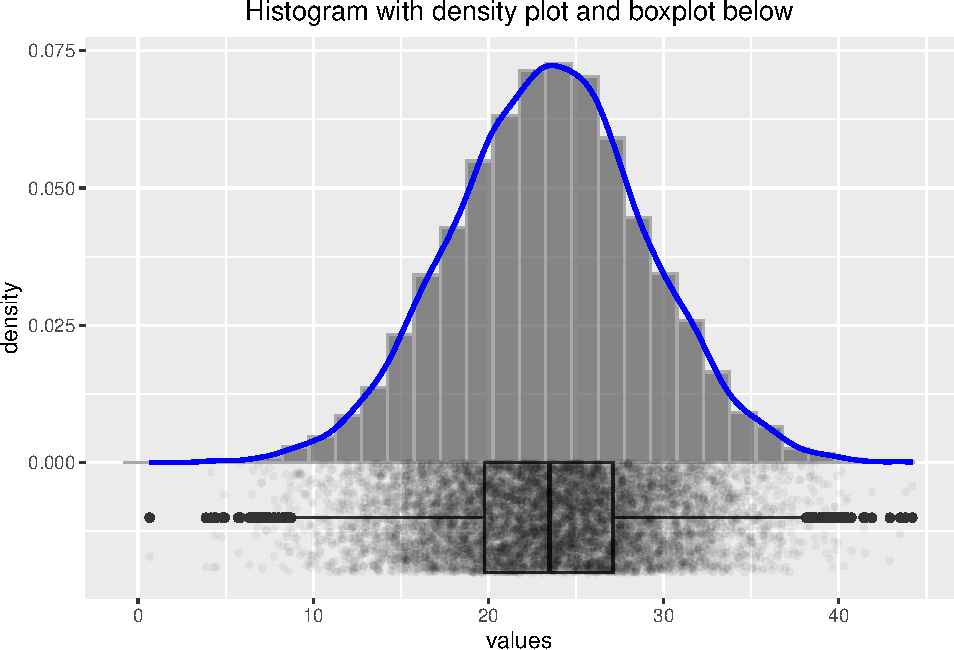
\includegraphics[keepaspectratio]{_main_files/figure-latex/unnamed-chunk-17-1.pdf}}

Some researchers would discard the values below 10 and above 40 as outliers, but we know here
that the data points are perfectly legitimate.
One important thing we should be aware of in connection with small sample sizes ist
variability. Let's create not \(10000\) samples of a normally distributed variable, but only \(25\) samples:

\begin{Shaded}
\begin{Highlighting}[]
\CommentTok{\# Generate normally distributed sample}
\FunctionTok{set.seed}\NormalTok{(}\DecValTok{1245}\NormalTok{) }\CommentTok{\# to get the same plot every time}
\NormalTok{x }\OtherTok{\textless{}{-}} \FunctionTok{rnorm}\NormalTok{(}\DecValTok{25}\NormalTok{, }\AttributeTok{mean =} \FloatTok{23.4}\NormalTok{, }\AttributeTok{sd =} \FloatTok{5.6}\NormalTok{)}
\NormalTok{df }\OtherTok{\textless{}{-}} \FunctionTok{data.frame}\NormalTok{(}\AttributeTok{values =}\NormalTok{ x)}

\NormalTok{p2 }\OtherTok{\textless{}{-}} \FunctionTok{ggplot}\NormalTok{(df, }\FunctionTok{aes}\NormalTok{(}\AttributeTok{x =}\NormalTok{ values)) }\SpecialCharTok{+}
  \FunctionTok{geom\_histogram}\NormalTok{(}\FunctionTok{aes}\NormalTok{(}\AttributeTok{y =} \FunctionTok{after\_stat}\NormalTok{(density)),}
                 \AttributeTok{bins =} \DecValTok{30}\NormalTok{, }\AttributeTok{alpha =} \FloatTok{0.7}\NormalTok{, }\AttributeTok{color =} \StringTok{"darkgrey"}\NormalTok{) }\SpecialCharTok{+}
  \FunctionTok{geom\_density}\NormalTok{(}\FunctionTok{aes}\NormalTok{(}\AttributeTok{y =} \FunctionTok{after\_stat}\NormalTok{(density)), }\AttributeTok{color =} \StringTok{"blue"}\NormalTok{, }\AttributeTok{linewidth =} \DecValTok{1}\NormalTok{) }\SpecialCharTok{+}
  \FunctionTok{geom\_boxplot}\NormalTok{(}\FunctionTok{aes}\NormalTok{(}\AttributeTok{y =} \SpecialCharTok{{-}}\FloatTok{0.01}\NormalTok{, }\AttributeTok{x =}\NormalTok{ values), }\AttributeTok{width =} \FloatTok{0.02}\NormalTok{,}
               \AttributeTok{position =} \FunctionTok{position\_nudge}\NormalTok{(}\AttributeTok{y =} \SpecialCharTok{{-}}\FloatTok{0.00}\NormalTok{)) }\SpecialCharTok{+}
  \FunctionTok{geom\_point}\NormalTok{(}\FunctionTok{aes}\NormalTok{(}\AttributeTok{y =} \SpecialCharTok{{-}}\FloatTok{0.01}\NormalTok{),}
             \AttributeTok{position =} \FunctionTok{position\_jitter}\NormalTok{(}\AttributeTok{width =} \FloatTok{0.002}\NormalTok{, }\AttributeTok{height =} \FloatTok{0.01}\NormalTok{),}
             \AttributeTok{size =} \DecValTok{1}\NormalTok{, }\AttributeTok{alpha =} \FloatTok{0.05}\NormalTok{) }\SpecialCharTok{+}
  \FunctionTok{ggtitle}\NormalTok{(}\StringTok{"Histogram with density plot and boxplot below"}\NormalTok{) }\SpecialCharTok{+}
  \FunctionTok{theme}\NormalTok{(}\AttributeTok{plot.title =} \FunctionTok{element\_text}\NormalTok{(}\AttributeTok{hjust =} \FloatTok{0.5}\NormalTok{))}
\NormalTok{p2}
\end{Highlighting}
\end{Shaded}

\pandocbounded{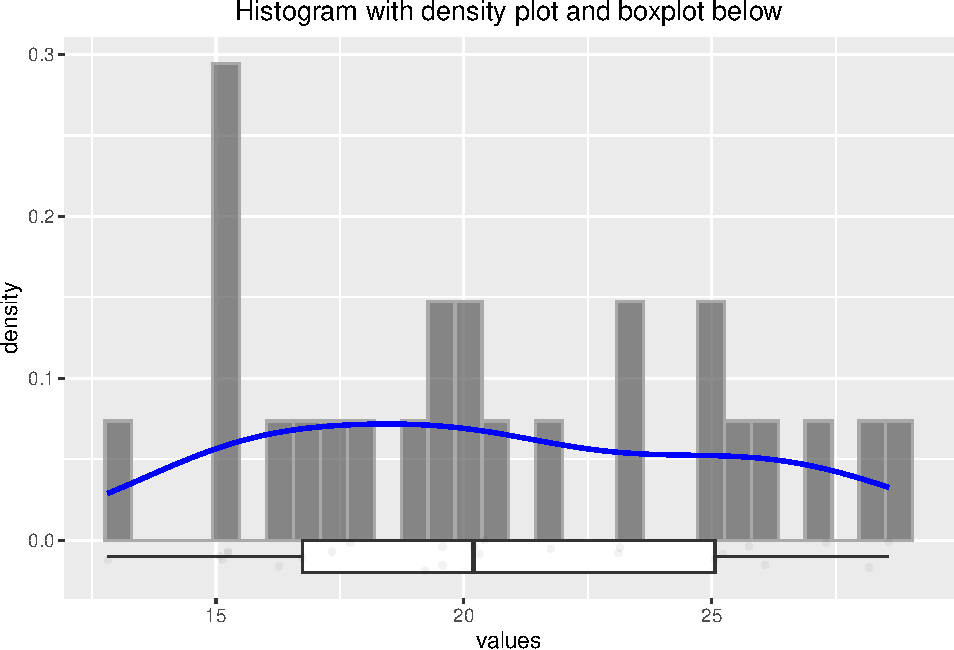
\includegraphics[keepaspectratio]{_main_files/figure-latex/unnamed-chunk-18-1.pdf}}

We \emph{know} (in this case) that these values come from a normal distribution with a mean
of \(23.4\) and a standard deviation of \(5.6\). Let's \emph{estimate} the parameters (\(\mu\), \(\sigma\)) from the sample
and use the often but not recommended Shapiro-wilk test for normality:

\begin{Shaded}
\begin{Highlighting}[]
\CommentTok{\# Estimate mean and standard deviation}
\FunctionTok{mean}\NormalTok{(x) }\CommentTok{\# or}
\end{Highlighting}
\end{Shaded}

\begin{verbatim}
## [1] 20.6017
\end{verbatim}

\begin{Shaded}
\begin{Highlighting}[]
\DecValTok{1} \SpecialCharTok{/} \FunctionTok{length}\NormalTok{(x) }\SpecialCharTok{*} \FunctionTok{sum}\NormalTok{(x)}
\end{Highlighting}
\end{Shaded}

\begin{verbatim}
## [1] 20.6017
\end{verbatim}

\begin{Shaded}
\begin{Highlighting}[]
\FunctionTok{sd}\NormalTok{(x) }\CommentTok{\# or}
\end{Highlighting}
\end{Shaded}

\begin{verbatim}
## [1] 4.622042
\end{verbatim}

\begin{Shaded}
\begin{Highlighting}[]
\FunctionTok{sqrt}\NormalTok{(}\DecValTok{1} \SpecialCharTok{/}\NormalTok{ (}\FunctionTok{length}\NormalTok{(x) }\SpecialCharTok{{-}} \DecValTok{1}\NormalTok{) }\SpecialCharTok{*} \FunctionTok{sum}\NormalTok{((x }\SpecialCharTok{{-}} \FunctionTok{mean}\NormalTok{(x))}\SpecialCharTok{\^{}}\DecValTok{2}\NormalTok{))}
\end{Highlighting}
\end{Shaded}

\begin{verbatim}
## [1] 4.622042
\end{verbatim}

\begin{Shaded}
\begin{Highlighting}[]
\FunctionTok{shapiro.test}\NormalTok{(x)}
\end{Highlighting}
\end{Shaded}

\begin{verbatim}
## 
##  Shapiro-Wilk normality test
## 
## data:  x
## W = 0.95059, p-value = 0.2585
\end{verbatim}

Firstly, the histogram looks rather differently when using a different \href{https://r-coder.com/set-seed-r/}{seed}. Secondly, we would probability
not be able to tell if the data stems from a normal distribution. Thirdly, the sample mean and standard deviation
are not all that bad estimators for the true (but unknown) mean and standard deviation. Nicely enough,
the Shapiro test would not reject the null hypothesis of normality in this case.

Let's try the Shapiro test with a t-distribution with 3 degrees of freedom, which is not normal:

\begin{Shaded}
\begin{Highlighting}[]
\FunctionTok{set.seed}\NormalTok{(}\DecValTok{1245}\NormalTok{) }\CommentTok{\# to get the same plot every time}
\NormalTok{x }\OtherTok{\textless{}{-}} \FunctionTok{rt}\NormalTok{(}\DecValTok{25}\NormalTok{, }\AttributeTok{df =} \DecValTok{3}\NormalTok{) }\CommentTok{\# random numbers from t{-}distribution}
\NormalTok{df }\OtherTok{\textless{}{-}} \FunctionTok{data.frame}\NormalTok{(}\AttributeTok{values =}\NormalTok{ x)}

\NormalTok{p2 }\OtherTok{\textless{}{-}} \FunctionTok{ggplot}\NormalTok{(df, }\FunctionTok{aes}\NormalTok{(}\AttributeTok{x =}\NormalTok{ values)) }\SpecialCharTok{+}
  \FunctionTok{geom\_histogram}\NormalTok{(}\FunctionTok{aes}\NormalTok{(}\AttributeTok{y =} \FunctionTok{after\_stat}\NormalTok{(density)),}
                 \AttributeTok{bins =} \DecValTok{30}\NormalTok{, }\AttributeTok{alpha =} \FloatTok{0.7}\NormalTok{, }\AttributeTok{color =} \StringTok{"darkgrey"}\NormalTok{) }\SpecialCharTok{+}
  \FunctionTok{geom\_density}\NormalTok{(}\FunctionTok{aes}\NormalTok{(}\AttributeTok{y =} \FunctionTok{after\_stat}\NormalTok{(density)), }\AttributeTok{color =} \StringTok{"blue"}\NormalTok{, }\AttributeTok{linewidth =} \DecValTok{1}\NormalTok{) }\SpecialCharTok{+}
  \FunctionTok{geom\_boxplot}\NormalTok{(}\FunctionTok{aes}\NormalTok{(}\AttributeTok{y =} \SpecialCharTok{{-}}\FloatTok{0.01}\NormalTok{, }\AttributeTok{x =}\NormalTok{ values), }\AttributeTok{width =} \FloatTok{0.02}\NormalTok{,}
               \AttributeTok{position =} \FunctionTok{position\_nudge}\NormalTok{(}\AttributeTok{y =} \SpecialCharTok{{-}}\FloatTok{0.00}\NormalTok{)) }\SpecialCharTok{+}
  \FunctionTok{geom\_point}\NormalTok{(}\FunctionTok{aes}\NormalTok{(}\AttributeTok{y =} \SpecialCharTok{{-}}\FloatTok{0.01}\NormalTok{),}
             \AttributeTok{position =} \FunctionTok{position\_jitter}\NormalTok{(}\AttributeTok{width =} \FloatTok{0.002}\NormalTok{, }\AttributeTok{height =} \FloatTok{0.01}\NormalTok{),}
             \AttributeTok{size =} \DecValTok{1}\NormalTok{, }\AttributeTok{alpha =} \FloatTok{0.05}\NormalTok{) }\SpecialCharTok{+}
  \FunctionTok{ggtitle}\NormalTok{(}\StringTok{"Histogram with density plot and boxplot below"}\NormalTok{) }\SpecialCharTok{+}
  \FunctionTok{theme}\NormalTok{(}\AttributeTok{plot.title =} \FunctionTok{element\_text}\NormalTok{(}\AttributeTok{hjust =} \FloatTok{0.5}\NormalTok{))}
\NormalTok{p2}
\end{Highlighting}
\end{Shaded}

\pandocbounded{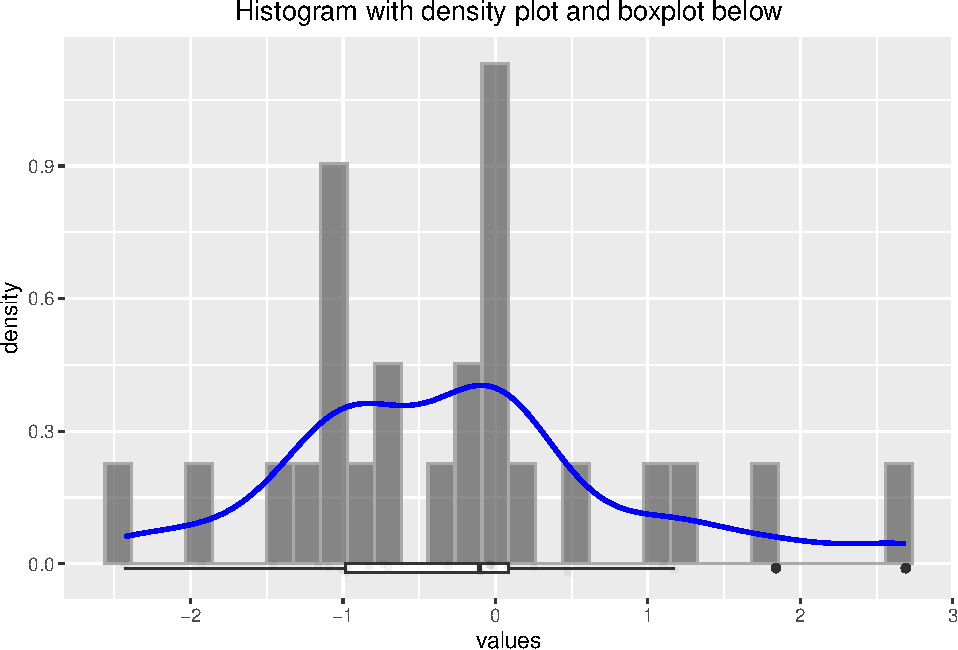
\includegraphics[keepaspectratio]{_main_files/figure-latex/unnamed-chunk-20-1.pdf}}

\begin{Shaded}
\begin{Highlighting}[]
\FunctionTok{shapiro.test}\NormalTok{(x)}
\end{Highlighting}
\end{Shaded}

\begin{verbatim}
## 
##  Shapiro-Wilk normality test
## 
## data:  x
## W = 0.95827, p-value = 0.3811
\end{verbatim}

Some researchers would argue, that the distribution is normal (since the p-value is rather large),
but we know it is not. We will be cautious with such ugly rule of thumbs.

\subsection{Example in the wild}\label{example-in-the-wild}

We will try to catch a histogram in the \emph{wild} (= in a research paper): We find one
\href{https://bmjopen.bmj.com/content/bmjopen/9/4/e023341.full.pdf}{here}.
\href{https://bmjopen.bmj.com/content/bmjopen/9/4/e023341/F1.large.jpg}{Figure 1} shows a histogram often
the foot posture index (FPI-6) scores from the participants (3217 healthy children aged 3 to 15).
``The FPI score may range from −12 (highly supinated) to +12 (highly pronated)''.
There are a few things to note here:

\begin{itemize}
\item
  Acccording to the Methods-section:
  ``Testing for normality using a Kolmogorov-Smirnov test,
  found non-normal distribution of all data\ldots{}''.
  Especially the BMI could be asymmetrically distributed, or also age. Unfortunately, we do not have
  histograms or boxplots for these variables. Nevertheless, the authors present the mean and standard deviation
  for these variables which implies (when not reading the methods section) that the data is (at least sufficiently)
  normally distributed.
\item
  Strictly speaking, an FPI score cannot be normally distributed since it takes discrete values which are bounded
  between -12 and 12 (normal distribution can take values between \(-\infty\) and \(\infty\)). But that should not be a problem with so many levels of an ordered categorical variable.
  It should be a sufficient approximation.
\item
  ``The FPI was analysed as continuous data, rather than as z-score data''.
  \href{https://www.youtube.com/watch?v=5S-Zfa-vOXs&ab_channel=KhanAcademy}{z-scores are standardized scores}:
  \[Z = \frac{X - \mu_X}{\sigma_X}\]
  Doing this for the FPI scores would give (FPI right, see Table 1):
  \[z_i = \frac{FPI_i - \overline{FPI}}{SD(FPI)} = \frac{FPI_i - 4.20}{3.00}\]
  \(\overline{FPI}\) ist the arithmetic mean of the FPI scores, \(SD(FPI)\) the standard deviation of the FPI scores.
  \(\mu_X\) is the expectation of X and \(\sigma_X\) the standard deviation of X.
  So we measure not in FPI units anymore, but in \textbf{standard deviations from the mean} which makes
  it easier to compare different variables with each other. A nice property is: If X is normally
  distributed (\(X \sim N(\mu, \sigma\))), then the z-scores are standard normally distributed (\(Z \sim N(0,1\))).
  See \hyperref[exercise4_descriptive_stats]{Exercise 4}. Of course \emph{both}, z-scores as well as FPI scores are
  considered ``continuous'' (in this context).
\item
  With so many obsvervations (\(n=3217\)), how would a truly normal distribution with the parameters
  \(FPI \sim N(4.20, 3.00)\) look like? We can simulate this with the following code:
\end{itemize}

\begin{Shaded}
\begin{Highlighting}[]
\FunctionTok{set.seed}\NormalTok{(}\DecValTok{8345}\NormalTok{) }\CommentTok{\# to get the same plot every time}
\NormalTok{x }\OtherTok{\textless{}{-}} \FunctionTok{rnorm}\NormalTok{(}\DecValTok{3217}\NormalTok{, }\AttributeTok{mean =} \FloatTok{4.20}\NormalTok{, }\AttributeTok{sd =} \FloatTok{3.00}\NormalTok{)}
\NormalTok{df }\OtherTok{\textless{}{-}} \FunctionTok{data.frame}\NormalTok{(}\AttributeTok{values =}\NormalTok{ x)}

\NormalTok{p2 }\OtherTok{\textless{}{-}} \FunctionTok{ggplot}\NormalTok{(df, }\FunctionTok{aes}\NormalTok{(}\AttributeTok{x =}\NormalTok{ values)) }\SpecialCharTok{+}
  \FunctionTok{geom\_histogram}\NormalTok{(}\FunctionTok{aes}\NormalTok{(}\AttributeTok{y =} \FunctionTok{after\_stat}\NormalTok{(density)),}
                 \AttributeTok{bins =} \DecValTok{30}\NormalTok{, }\AttributeTok{alpha =} \FloatTok{0.7}\NormalTok{, }\AttributeTok{color =} \StringTok{"darkgrey"}\NormalTok{) }\SpecialCharTok{+}
  \FunctionTok{geom\_density}\NormalTok{(}\FunctionTok{aes}\NormalTok{(}\AttributeTok{y =} \FunctionTok{after\_stat}\NormalTok{(density)), }\AttributeTok{color =} \StringTok{"blue"}\NormalTok{, }\AttributeTok{linewidth =} \DecValTok{1}\NormalTok{) }\SpecialCharTok{+}
  \FunctionTok{geom\_boxplot}\NormalTok{(}\FunctionTok{aes}\NormalTok{(}\AttributeTok{y =} \SpecialCharTok{{-}}\FloatTok{0.01}\NormalTok{, }\AttributeTok{x =}\NormalTok{ values), }\AttributeTok{width =} \FloatTok{0.02}\NormalTok{,}
               \AttributeTok{position =} \FunctionTok{position\_nudge}\NormalTok{(}\AttributeTok{y =} \SpecialCharTok{{-}}\FloatTok{0.00}\NormalTok{)) }\SpecialCharTok{+}
  \FunctionTok{geom\_point}\NormalTok{(}\FunctionTok{aes}\NormalTok{(}\AttributeTok{y =} \SpecialCharTok{{-}}\FloatTok{0.01}\NormalTok{),}
             \AttributeTok{position =} \FunctionTok{position\_jitter}\NormalTok{(}\AttributeTok{width =} \FloatTok{0.002}\NormalTok{, }\AttributeTok{height =} \FloatTok{0.01}\NormalTok{),}
             \AttributeTok{size =} \DecValTok{1}\NormalTok{, }\AttributeTok{alpha =} \FloatTok{0.05}\NormalTok{) }\SpecialCharTok{+}
  \FunctionTok{ggtitle}\NormalTok{(}\StringTok{"Histogram with density plot and boxplot below"}\NormalTok{) }\SpecialCharTok{+}
  \FunctionTok{theme}\NormalTok{(}\AttributeTok{plot.title =} \FunctionTok{element\_text}\NormalTok{(}\AttributeTok{hjust =} \FloatTok{0.5}\NormalTok{))}
\NormalTok{p2}
\end{Highlighting}
\end{Shaded}

\pandocbounded{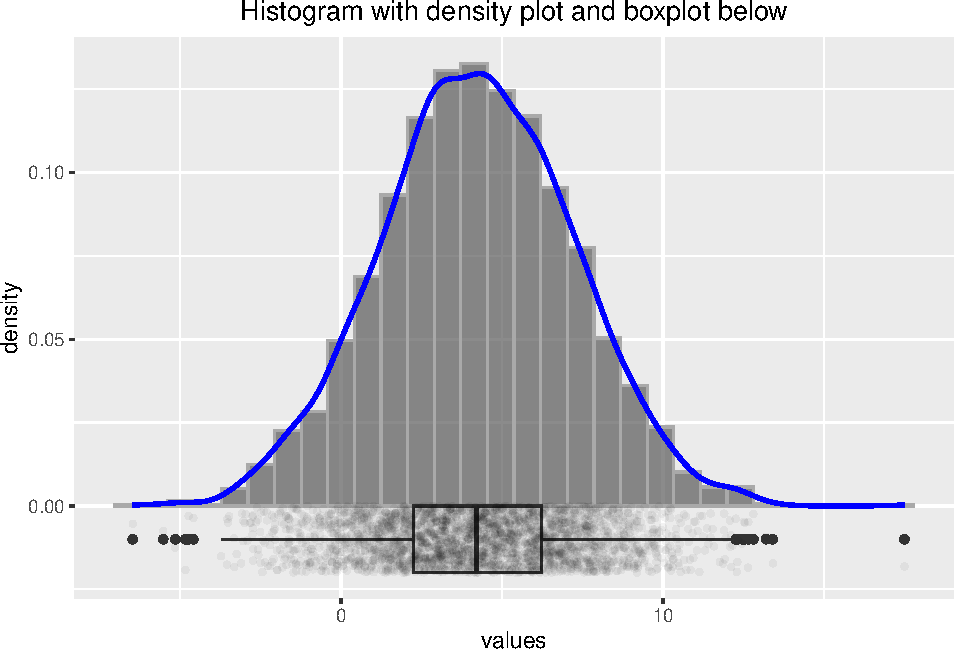
\includegraphics[keepaspectratio]{_main_files/figure-latex/unnamed-chunk-21-1.pdf}}

Comparing these histograms (using different seed-values), we could assume that for truly normally distributed
FPI scores, the histogram might look smoother than the one in Figure 1 in the paper. Especially the values around 6
seem to deviate from the normal distribution.

\section{Correlation}\label{correlation}

The \href{https://en.wikipedia.org/wiki/Correlation}{correlation} between two variables is a measure
of the strength and direction of the \textbf{linear} relationship between them. It does \textbf{not} (directly)
a measure of other kinds of relationships (for instance monotonic or polynomial).
See also \href{https://en.wikipedia.org/wiki/Anscombe\%27s_quartet}{Anscombe's quartet}.

Correlation is often denoted by the Greek letter

\[\rho = \frac{\text{Cov}(X, Y)}{\sigma_X \sigma_Y}\]
for the population parameter (the true but unknown)

where:

\begin{itemize}
\item
  \(\text{Cov}(X, Y)\) is the covariance between variables \(X\) and \(Y\),
\item
  \(\sigma_X\) and \(\sigma_Y\) are the population standard deviations of \(X\) and \(Y\), respectively.
\end{itemize}

and

\[r = \frac{\sum (X_i - \bar{X})(Y_i - \bar{Y})}{\sqrt{\sum (X_i - \bar{X})^2 \sum (Y_i - \bar{Y})^2}}\]

for the sample estimate.

\textbf{Remember: We use \(r\) to estimate \(\rho\) using the sample.}

The correlation coefficient can take values between -1 and 1.

\begin{itemize}
\item
  A value of 1 indicates a perfect positive linear relationship between the variables.
\item
  A value of -1 indicates a perfect negative linear relationship between the variables.
\end{itemize}

See \href{https://en.wikipedia.org/wiki/Correlation\#/media/File:Correlation_examples2.svg}{here} and
\href{https://en.wikipedia.org/wiki/Correlation\#/media/File:Pearson_Correlation_Coefficient_and_associated_scatterplots.png}{here}
for a nice illustration. Study this in detail. A correlation of \(\pm 1\) just means that the data points lie on a straight line.
It does not say anything about the steepness of the line.

You can watch these videos to get a better understanding of the concept:

\begin{itemize}
\item
  \href{https://www.youtube.com/watch?v=xZ_z8KWkhXE&ab_channel=StatQuestwithJoshStarmer}{StatQuest - correlation}
\item
  \href{https://www.youtube.com/watch?v=qtaqvPAeEJY&ab_channel=StatQuestwithJoshStarmer}{StatQuest - covariance}
\item
  \href{https://www.youtube.com/watch?v=rijqfllOq6g&ab_channel=3-MinuteDataScience}{Animated correlation}
\end{itemize}

Correlation is an often (over-)used measure in research.
It is important to note that
\href{https://en.wikipedia.org/wiki/Correlation_does_not_imply_causation}{correlation does not imply causation}.
For instance,
\href{https://www.sciencedirect.com/science/article/pii/S2590291120300711}{chocolate consumption is positively correlated with the number of Nobel laureates} in a country.
This does - unfortunately - not mean that eating chocolate makes you smarter.

One thing many of us think when they see a high correlation (near 1) is that if we know the value of one variable,
we can predict the value of the other variable. This is not necessarily true.
This \href{https://en.wikipedia.org/wiki/Pearson_correlation_coefficient\#Interpretation}{section} explains why.
Study the visualization \href{https://en.wikipedia.org/wiki/Pearson_correlation_coefficient\#/media/File:Pearson_correlation_and_prediction_intervals.svg}{here}.
It depicts the reduction of the prediction interval for Y given X as the correlation
increases (assuming that the variables are jointly normally distributed). \textbf{How much smaller is the interval where my next observation of Y
will fall if I know the value of X?} As you can see, this curve is relatively flat in the beginning, meaning, on an individual level,
the correlation does not tell us much about the value of Y given X.
Of course with correlation 1, we can predict the value of Y perfectly, but even with a correlation of 0.5
(which is considered high in many areas), the prediction interval for Y is only 13\% smaller.

One often reads that the two variables used for calculation of a
\href{https://en.wikipedia.org/wiki/Pearson_correlation_coefficient}{Pearson correlation coefficient} should be normally distributed.
This is not necessary, at least not for descriptive purposes. The correlation coefficient is a measure of the linear relationship
and we can think of an example with skewed data where the correlation coefficient is still meaningful:

\begin{Shaded}
\begin{Highlighting}[]
\CommentTok{\# Load required libraries}
\FunctionTok{library}\NormalTok{(ggplot2)}
\FunctionTok{library}\NormalTok{(ggExtra)}

\CommentTok{\# Set seed for reproducibility}
\FunctionTok{set.seed}\NormalTok{(}\DecValTok{1234}\NormalTok{)}

\CommentTok{\# Parameters}
\NormalTok{n }\OtherTok{\textless{}{-}} \DecValTok{200}  \CommentTok{\# Sample size}
\NormalTok{beta }\OtherTok{\textless{}{-}} \FloatTok{0.7}  \CommentTok{\# Desired beta}

\CommentTok{\# Generate left{-}skewed variable x (negative exponential distribution)}
\NormalTok{x }\OtherTok{\textless{}{-}} \SpecialCharTok{{-}}\FunctionTok{rexp}\NormalTok{(n, }\AttributeTok{rate =} \DecValTok{1}\NormalTok{)}

\CommentTok{\# Generate correlated left{-}skewed variable y}
\NormalTok{error }\OtherTok{\textless{}{-}} \FunctionTok{rnorm}\NormalTok{(n, }\AttributeTok{mean =} \DecValTok{0}\NormalTok{, }\AttributeTok{sd =} \DecValTok{2}\NormalTok{)}
\NormalTok{y }\OtherTok{\textless{}{-}}\NormalTok{ beta }\SpecialCharTok{*}\NormalTok{ x }\SpecialCharTok{+}\NormalTok{ error}

\CommentTok{\# Create a data frame}
\NormalTok{data }\OtherTok{\textless{}{-}} \FunctionTok{data.frame}\NormalTok{(}\AttributeTok{x =}\NormalTok{ x, }\AttributeTok{y =}\NormalTok{ y)}

\CommentTok{\# Create scatterplot with marginal histograms and trendline}
\NormalTok{p }\OtherTok{\textless{}{-}} \FunctionTok{ggplot}\NormalTok{(data, }\FunctionTok{aes}\NormalTok{(}\AttributeTok{x =}\NormalTok{ x, }\AttributeTok{y =}\NormalTok{ y)) }\SpecialCharTok{+}
  \FunctionTok{geom\_point}\NormalTok{(}\AttributeTok{alpha =} \FloatTok{0.5}\NormalTok{, }\AttributeTok{color =} \StringTok{"blue"}\NormalTok{) }\SpecialCharTok{+}
  \FunctionTok{geom\_smooth}\NormalTok{(}\AttributeTok{method =} \StringTok{"lm"}\NormalTok{, }\AttributeTok{color =} \StringTok{"red"}\NormalTok{, }\AttributeTok{se =} \ConstantTok{FALSE}\NormalTok{) }\SpecialCharTok{+}
  \FunctionTok{labs}\NormalTok{(}\AttributeTok{title =} \StringTok{"Scatterplot with Left{-}Skewed x and y and Trendline"}\NormalTok{,}
       \AttributeTok{x =} \StringTok{"Left{-}Skewed x"}\NormalTok{, }\AttributeTok{y =} \StringTok{"y"}\NormalTok{) }\SpecialCharTok{+}
  \FunctionTok{theme\_minimal}\NormalTok{()}

\CommentTok{\# Add marginal histograms using ggExtra}
\NormalTok{ggExtra}\SpecialCharTok{::}\FunctionTok{ggMarginal}\NormalTok{(p, }\AttributeTok{type =} \StringTok{"histogram"}\NormalTok{, }\AttributeTok{fill =} \StringTok{"lightblue"}\NormalTok{, }\AttributeTok{color =} \StringTok{"black"}\NormalTok{)}
\end{Highlighting}
\end{Shaded}

\begin{verbatim}
## `geom_smooth()` using formula = 'y ~ x'
## `geom_smooth()` using formula = 'y ~ x'
## `geom_smooth()` using formula = 'y ~ x'
\end{verbatim}

\pandocbounded{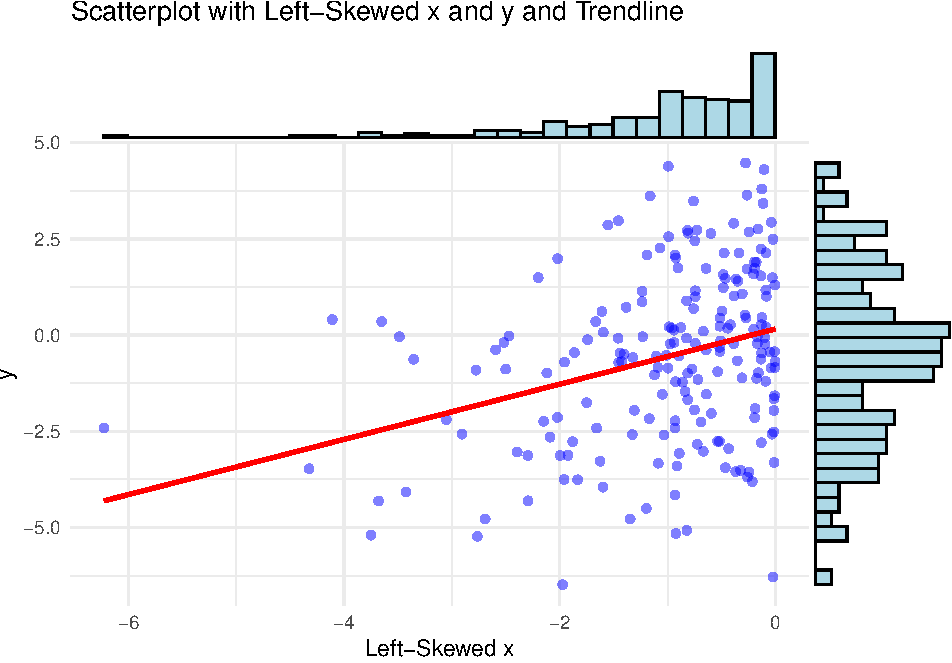
\includegraphics[keepaspectratio]{_main_files/figure-latex/unnamed-chunk-22-1.pdf}}

\emph{If} X and Y are bivariate normally distributed, then one can use the variable
\(t = r \sqrt{\frac{n-2}{1-r^2}}\) as test statistic for the null hypothesis (next chapter) \(H_0: \rho = 0\).
Note: It is not sufficient for X and Y to be individually normally distributed in order to
be \href{https://en.wikipedia.org/wiki/Multivariate_normal_distribution\#Bivariate_case}{jointly normally distributed}.

\subsection{Example in the wild}\label{example-in-the-wild-1}

Let's again visit the previous \href{https://bmjopen.bmj.com/content/9/4/e023341}{paper}.
In the results, correlations are presented in a dichotomous way with regards to p-values,
which should be \href{https://www.tandfonline.com/doi/full/10.1080/00031305.2019.1583913}{avoided}.
We will expand on this in the next chapter. For large sample sizes, even small (true) correlations will be ``significant'',
especially, if one decides to use an arbitrary threshold for the p-values like \(0.05\). There is not much information
in this fact. I would argue that all p-values for such large sample sizes and larger correlations do not carry much information.
See also \hyperref[exercise5_descriptive_stats]{Exercise 5}.

\textbf{That was all nice, what could go wrong?}

(The sample) Correlation (coefficient) is based (see the formula above) on the artihmetic mean \(\bar{X}\)
(capital X since we are talking about the
\href{https://www.youtube.com/watch?v=Y9nsL69CwbU&ab_channel=VeryNormal}{random variable} which is realised when
the \(X_i\) have materialized into the \(x_i\)) and sample standard deviation \(\sigma\).

The sample mean is not robust against outliers. A single large value can distort the mean arbitrarily much.
Hence, the correlation coefficient is not robust against outliers. Let's see this in action:

\begin{Shaded}
\begin{Highlighting}[]
\CommentTok{\# Load necessary libraries}
\FunctionTok{library}\NormalTok{(ggplot2)}
\FunctionTok{library}\NormalTok{(ggpubr)}

\CommentTok{\# Set seed for reproducibility}
\FunctionTok{set.seed}\NormalTok{(}\DecValTok{123}\NormalTok{)}

\CommentTok{\# Parameters}
\NormalTok{n }\OtherTok{\textless{}{-}} \DecValTok{100}  \CommentTok{\# Sample size}
\NormalTok{rho }\OtherTok{\textless{}{-}} \FloatTok{0.75}  \CommentTok{\# Desired correlation}

\CommentTok{\# Generate bivariate normal data with specified correlation}
\NormalTok{x }\OtherTok{\textless{}{-}} \FunctionTok{rnorm}\NormalTok{(n)}
\NormalTok{y }\OtherTok{\textless{}{-}}\NormalTok{ rho }\SpecialCharTok{*}\NormalTok{ x }\SpecialCharTok{+} \FunctionTok{sqrt}\NormalTok{(}\DecValTok{1} \SpecialCharTok{{-}}\NormalTok{ rho}\SpecialCharTok{\^{}}\DecValTok{2}\NormalTok{) }\SpecialCharTok{*} \FunctionTok{rnorm}\NormalTok{(n)}

\CommentTok{\# Store original data}
\NormalTok{data\_original }\OtherTok{\textless{}{-}} \FunctionTok{data.frame}\NormalTok{(}\AttributeTok{x =}\NormalTok{ x, }\AttributeTok{y =}\NormalTok{ y)}

\CommentTok{\# Function to create scatterplot with trend line and correlation}
\NormalTok{create\_plot }\OtherTok{\textless{}{-}} \ControlFlowTok{function}\NormalTok{(data, title) \{}
  \FunctionTok{ggplot}\NormalTok{(data, }\FunctionTok{aes}\NormalTok{(}\AttributeTok{x =}\NormalTok{ x, }\AttributeTok{y =}\NormalTok{ y)) }\SpecialCharTok{+}
    \FunctionTok{geom\_point}\NormalTok{(}\AttributeTok{alpha =} \FloatTok{0.6}\NormalTok{, }\AttributeTok{color =} \StringTok{"blue"}\NormalTok{) }\SpecialCharTok{+}
    \FunctionTok{geom\_smooth}\NormalTok{(}\AttributeTok{method =} \StringTok{"lm"}\NormalTok{, }\AttributeTok{se =} \ConstantTok{FALSE}\NormalTok{, }\AttributeTok{color =} \StringTok{"red"}\NormalTok{) }\SpecialCharTok{+}
    \FunctionTok{labs}\NormalTok{(}\AttributeTok{title =}\NormalTok{ title, }\AttributeTok{subtitle =} \FunctionTok{paste}\NormalTok{(}\StringTok{"Correlation:"}\NormalTok{,}
                                         \FunctionTok{round}\NormalTok{(}\FunctionTok{cor}\NormalTok{(data}\SpecialCharTok{$}\NormalTok{x, data}\SpecialCharTok{$}\NormalTok{y), }\DecValTok{2}\NormalTok{))) }\SpecialCharTok{+}
    \FunctionTok{theme\_minimal}\NormalTok{() }\SpecialCharTok{+}
    \FunctionTok{theme}\NormalTok{(}\AttributeTok{plot.title =} \FunctionTok{element\_text}\NormalTok{(}\AttributeTok{hjust =} \FloatTok{0.5}\NormalTok{))  }\CommentTok{\# Center the title}
\NormalTok{\}}

\CommentTok{\# Original scatterplot}
\NormalTok{p\_original }\OtherTok{\textless{}{-}} \FunctionTok{create\_plot}\NormalTok{(data\_original, }\StringTok{"Original Data"}\NormalTok{)}

\CommentTok{\# Add outlier in x}
\NormalTok{data\_outlier\_x }\OtherTok{\textless{}{-}}\NormalTok{ data\_original}
\NormalTok{data\_outlier\_x}\SpecialCharTok{$}\NormalTok{x[n] }\OtherTok{\textless{}{-}} \FunctionTok{max}\NormalTok{(x) }\SpecialCharTok{+} \DecValTok{5}  \CommentTok{\# Extreme value in x}
\NormalTok{p\_outlier\_x }\OtherTok{\textless{}{-}} \FunctionTok{create\_plot}\NormalTok{(data\_outlier\_x, }\StringTok{"Outlier in X"}\NormalTok{)}

\CommentTok{\# Add outlier in both x and y}
\NormalTok{data\_outlier\_xy }\OtherTok{\textless{}{-}}\NormalTok{ data\_original}
\NormalTok{data\_outlier\_xy}\SpecialCharTok{$}\NormalTok{x[n] }\OtherTok{\textless{}{-}} \FunctionTok{max}\NormalTok{(x) }\SpecialCharTok{+} \DecValTok{5}  \CommentTok{\# Extreme value in x}
\NormalTok{data\_outlier\_xy}\SpecialCharTok{$}\NormalTok{y[n] }\OtherTok{\textless{}{-}} \FunctionTok{max}\NormalTok{(y) }\SpecialCharTok{+} \DecValTok{5}  \CommentTok{\# Extreme value in y}
\NormalTok{p\_outlier\_xy }\OtherTok{\textless{}{-}} \FunctionTok{create\_plot}\NormalTok{(data\_outlier\_xy, }\StringTok{"Outlier in Both X and Y"}\NormalTok{)}

\CommentTok{\# Add outlier in y}
\NormalTok{data\_outlier\_y }\OtherTok{\textless{}{-}}\NormalTok{ data\_original}
\NormalTok{data\_outlier\_y}\SpecialCharTok{$}\NormalTok{y[n] }\OtherTok{\textless{}{-}} \FunctionTok{max}\NormalTok{(y) }\SpecialCharTok{+} \DecValTok{5}  \CommentTok{\# Extreme value in y}
\NormalTok{p\_outlier\_y }\OtherTok{\textless{}{-}} \FunctionTok{create\_plot}\NormalTok{(data\_outlier\_y, }\StringTok{"Outlier in Y"}\NormalTok{)}

\CommentTok{\# Arrange plots using ggarrange}
\FunctionTok{ggarrange}\NormalTok{(p\_original, p\_outlier\_x, p\_outlier\_xy, p\_outlier\_y,}
          \AttributeTok{labels =} \FunctionTok{c}\NormalTok{(}\StringTok{"A"}\NormalTok{, }\StringTok{"B"}\NormalTok{, }\StringTok{"C"}\NormalTok{, }\StringTok{"D"}\NormalTok{),}
          \AttributeTok{ncol =} \DecValTok{2}\NormalTok{, }\AttributeTok{nrow =} \DecValTok{2}\NormalTok{)}
\end{Highlighting}
\end{Shaded}

\begin{verbatim}
## `geom_smooth()` using formula = 'y ~ x'
## `geom_smooth()` using formula = 'y ~ x'
## `geom_smooth()` using formula = 'y ~ x'
## `geom_smooth()` using formula = 'y ~ x'
\end{verbatim}

\pandocbounded{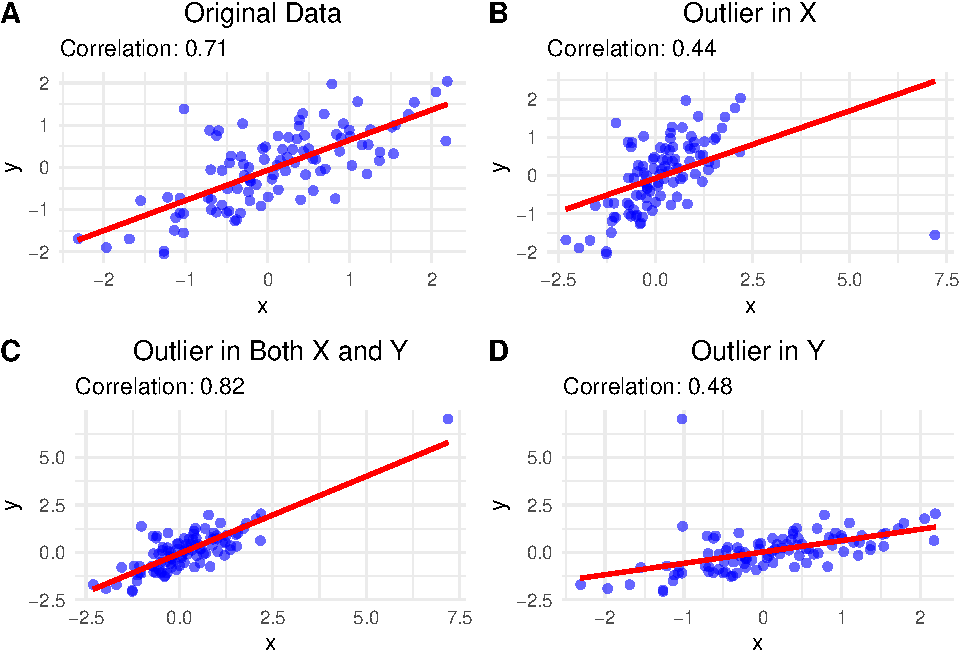
\includegraphics[keepaspectratio]{_main_files/figure-latex/unnamed-chunk-23-1.pdf}}

\begin{itemize}
\item
  A: \(r=0.71\) for the original data.
\item
  B: When we add an outlier in x, \(r\) decreases to \(0.44\) and the trendline is notably shifted.

  The reason for the smaller correlation is that the outlier is above the mean of the x values and below
  the mean of the y values and therefore adds negatively to the covariance.
\item
  C: When we add an outlier in both \(x\) and \(y\), \(r\) stays relatively stable.
  The reason is that the outlier is above the mean of the x values and above the mean of the y values,
  so it adds positively to the covariance. Also, the outlier is in line with the trend of the data.
  We could ask, what happend in this data point? Was another scale used for instance?
\item
  D: When we add an outlier in \(y\), the \(r\) decreases to 0.48.
  The reason for the smaller correlation is that the outlier is above the mean of the y values
  and below the mean of the x values and therefore adds negatively to the covariance.
\item
  We could also ask why the trend lines (created with simple linear regression) change the way they do.
  We will come to this later in our courses.
\end{itemize}

\section{Exercises}\label{exercises-1}

\subsection{Exercise 1 - Recreate table with fake data}\label{exercise-1---recreate-table-with-fake-data}

\begin{itemize}
\tightlist
\item
  Create fake data for the study mentioned \hyperref[example_study1_physio]{above} in R.
\item
  Recreate Table 2 of the paper mentioned \hyperref[example_study1_physio]{above} with fake data in R (using GPT, the R package \emph{gtsummary} and other useful packages).
  This is rather helpful later on in your master thesis.
\item
  Try to export the table to Excel and Word.
\end{itemize}

\subsection{Exercise 2 - Outliers and estimates}\label{exercise-2---outliers-and-estimates}

Let's assume we know that the \emph{Cognitive flexibility} is normally distributed with a mean of 60 and a standard deviation of 7.4 (Table 1): \(CognFlex \sim N(60,7.4)\).

\begin{itemize}
\tightlist
\item
  Draw a sample of 165 persons from this distribution and calculate the mean and standard deviation of the sample.
  How good is the estimate of the true (and in this case: known) mean and standard deviation?
\item
  Let's replace some of the data points with outliers. Change the score of 5 persons with to impossible CognFlex score of 100.
  Calculate the mean and standard deviation of the sample. How do the estimates change?
\item
  When we try to estimate the location of our \emph{Cognitive flexibility} distribution with the median,
  how many outliers of what magnitude are necessary to disturb the estimate by 5 points?
\end{itemize}

\subsection{Exercise 3 - Recreating data in Table 2}\label{exercise3_descriptive_stats}

We assume that \emph{age} in both groups is normally distributed with a mean of 48 (47) years
and a standard deviation of 16 (15) years:

\(Age_{UsualCare} \sim Normal(\mu = 48, \sigma = 16)\) and

\(Age_{CFT} \sim Normal(\mu = 47,\sigma = 15)\).

\begin{itemize}
\tightlist
\item
  Under these assumptions, what is the probability, that we would see a person of age 60 or older in a new sample (in either group)?
\item
  What is the probability, that we would see a person of age 18 or younger in a new sample?
\item
  Give a 99\% interval for the age in CFT,
  where we would expect a new person drawn from the same population.
\end{itemize}

Let's assume \emph{Sex} is binomially distributed with a probability of \(p = 0.59\) for both groups.

\begin{itemize}
\tightlist
\item
  What is the probability, that we would see a woman as the next recruited person in the \emph{Usual care} group?
\item
  What is the probability, that we would see no man in a sample of 10 persons in the \emph{CFT} group?
\item
  Sometimes you want balanced samples. How many patients would we need to recruit to get at least 45 women with a probability of at least 90\%.
  (We could solve this with simulation.)
\end{itemize}

\subsection{Exercise 4 - Z-scores}\label{exercise4_descriptive_stats}

\begin{itemize}
\tightlist
\item
  Show with a simulation that the z-scores are standard normally distributed if the original variable is normally distributed.
\item
  Try different parameter values for \(\mu\) and \(\sigma\) and plot the histogram of the z-scores.
\item
  Optional: Try to prove this mathematically.
\end{itemize}

\subsection{Exercise 5 - Correlation}\label{exercise5_descriptive_stats}

The following R-code creates correlated samples with a (true) correlation \(\rho\):

\begin{Shaded}
\begin{Highlighting}[]
\FunctionTok{set.seed}\NormalTok{(}\DecValTok{1234}\NormalTok{)}
\NormalTok{n }\OtherTok{\textless{}{-}} \DecValTok{1000}
\NormalTok{rho }\OtherTok{\textless{}{-}} \FloatTok{0.5}
\NormalTok{x }\OtherTok{\textless{}{-}} \FunctionTok{rnorm}\NormalTok{(n)}
\NormalTok{y }\OtherTok{\textless{}{-}}\NormalTok{ rho }\SpecialCharTok{*}\NormalTok{ x }\SpecialCharTok{+} \FunctionTok{sqrt}\NormalTok{(}\DecValTok{1} \SpecialCharTok{{-}}\NormalTok{ rho}\SpecialCharTok{\^{}}\DecValTok{2}\NormalTok{) }\SpecialCharTok{*} \FunctionTok{rnorm}\NormalTok{(n)}
\FunctionTok{cor}\NormalTok{(x, y)}
\end{Highlighting}
\end{Shaded}

\begin{verbatim}
## [1] 0.541743
\end{verbatim}

\begin{itemize}
\tightlist
\item
  Try different values for \(\rho\) and \(n\) and plot the scatterplot of \(x\) and \(y\).
\item
  Execute the code above 1000 times and save the correlation coefficient in a vector.
\item
  Calculate the sample quantiles and interquantile range of the simulated correlation coefficients.
  What do you observe with respect to variability?
\item
  Plot the histogram of the simulated correlation coefficients.
\end{itemize}

\section{Solutions}\label{solutions-1}

Solutions for this chapter can be found \href{https://github.com/jdegenfellner/Script_QM1_ZHAW/tree/main/Solutions_to_Exercises/3_Descriptive_statistics}{here}.

  \bibliography{book.bib,packages.bib}

\end{document}
